\begin{refsection}
%!TEX root = ../thesis.tex
%*******************************************************************************
%****************************** Third Chapter **********************************
%*******************************************************************************
\chapter{Metal Contacts to Phosphorous Doped Diamond}
\label{ch:electrical_experiments}
% **************************** Define Graphics Path **************************
\ifpdf
    \graphicspath{{Chapter3/Figs/Raster/}{Chapter3/Figs/PDF/}{Chapter3/Figs/}}
\else
    \graphicspath{{Chapter3/Figs/Vector/}{Chapter3/Figs/}}
\fi

\section{Introduction}
\subsection{Background}
Diamond offers exceptional material properties for electrical devices that are unparalleled by other wide bandgap semiconductors. In the creation of devices that rely upon n and p-type doping however, many challenges arise from the limitations that diamond imposes upon device fabrication. Due to its extraordinary hardness and densely packed crystal lattice, doping via implantation has had marginal success \cite{Das2022-1} and CVD growth is the preferred choice for doped material \cite{Yang2021}. The selection of donor candidates is limited, with nitrogen forming a deep donor level of around 1.6--1.7 \si{\electronvolt} \cite{li1998} due to a chemical re-bonding of the donor electron on a neighbouring carbon atom simultaneous with a lone-pair on the nitrogen atom itself \cite{goss2008}. Phosphorous, despite having a lower solubility than nitrogen within the diamond lattice, is able to provide a shallower donor level at around 0.57--0.60 \si{\electronvolt} \cite{koizumi2000}. Various strategies of co-doping phosphorous with other elements have been examined theoretically such as in \cite{alfieri2018}, but experimentally, substitutional phosphorous remains the only bulk n-type donor within diamond. The maximum dopant concentration depends primarily on the crystal orientation, with the \hkl{111} orientation providing the highest observed concentrations of around $1\times10^{20}$ \si{\atoms\per\centi\metre\cubed} \cite{grotjohn2014}. Boron doped p-type material is most readily deposited onto the \hkl{100} orientation, in large part due to the ready incorporation of crystalline defects on the \hkl{111} orientation. Typical Hall mobility measurements for boron doped diamond at room temperature on \hkl{111} oriented samples are around 500 \si{\cm\squared\per\volt\per\second} as seen in \cite{ri2005} while on \hkl{100} oriented samples the Hall carrier mobility reaches 2000 \si{\cm\squared\per\volt\per\second} as demonstrated by \cite{mortet2008}. These defects in \hkl{111} oriented diamond growth have led to significant efforts in the improvement of \hkl{100} oriented phosphorous doped CVD growth, with concentrations in the range of $10^{16}-10^{18}$ \cite{kato2007}. However, high compensation ratios become a significant limiting factor in phosphorous doped films grown on \hkl{100} oriented substrates as investigated more recently by \cite{stenger2021}.

\subsection{Ohmic Contact Formation to Diamond Devices}
One common theme throughout the development of diamond based electronic devices is the challenge of ohmic contact formation, as well as reliable Schottky contacts. This is in large part due to the presence of significant charge screening, resulting in strong Fermi level pinning at the diamond surface in both boron \cite{baker1993} and phosphorous \cite{suzuki2006} doped samples. This is a significant issue for devices that require phosphorous doped diamond, due to the significant activation energy required for carrier promotion. While boron doped diamond can reach a metallic level at around $10^{20}$ \si{\atoms\per\centi\metre\cubed}, allowing for high quality ohmic contact formation via annealed titanium with standard capping layers of gold or platinum/gold, this is not the case for phosphorous doping without novel approaches \cite{valappil2023}. This can be expressed with the ideal theory of metal to n-type semiconductor contacts, in which the contact resistivity $\rho_{c}$ varies exponentially by the factor $\frac{\phi_{b}}{\sqrt{N_{D}}}$ where $\phi_{b}$ is the Schottky barrier height and $N_{D}$ is the active donor concentration. Since it is difficult to deviate from the Fermi level pinning of $\sim4.3$ \si{\electronvolt} below the conduction band, instead the approach to reduce contact resistivity is to increase the doping concentration $N_{D}$. This has previously been used to great effect in boron doped diamond, where the Fermi level pinning of oxygen terminated diamond relative to the valence band is around $1.3$ \si{\electronvolt} \cite{yamanaka2000} and has the same issues with regards to the independence of Schottky barrier height from metal contact work functions. With boron doping of $2\text{\textendash}6\times10^{17}$ \si{\atoms\per\centi\metre\cubed}, specific contact resistivities of $1.3\times10^{-5}$ \si{\ohm\centi\metre\squared} have been demonstrated using annealed Ti contacts \cite{chen2005}.

%Ushizawa1998 compared boron growth of 100 and 111 - 111 better for high boron dopant? higher concentration on 111 anyway - preferential growth in high boron conditions. same for phosphorous then? only the crystalline quality that might be a massive factor for 100 samples versus 111 but also we don't need such high concentrations of boron so I guess 10^19 on 100 is more than enough lol. Only an issue for my deep trap 0.6ev phosphorous.... large differences in the growth mechanism too, high methane produces better samples on 111 - ri2005, opposite for 10? 
\subsection{Overview of Methodology and Novel Techniques}
In this chapter, various experimental characterisation methods have been employed to investigate the properties of heavily phosphorous doped diamond as used in ohmic contact fabrication. Recent efforts such as that of \cite{abubakr2022} in laser-induced ohmic contact formation for diamond detector charge collectors and \cite{valappil2023} in corrosion-resistive coaxial arc plasma deposited nanocarbon electrodes clearly demonstrate the ongoing development of phosphorous based devices, with a heavy focus on new methods for forming ohmic contacts in various device structures.

Through standard photolithography and metal deposition, simple Ti/Au and Ti/Pt/Au contacts were investigated and studied across a wide range of temperatures. Differences in the annealing conditions as well as the quality of the photolithography resulted in quite different experimental observations for this material. To understand the possible causes of some of these differences, other material characterisation methods are performed to help elucidate on the nature of heavily phosphorous doped diamond such as secondary ion mass spectroscopy (SIMS), X-ray photoelectron spectroscopy (XPS), atomic force microscopy (AFM) and optical microscopy.

Then, another avenue to improve the characteristics of ohmic contacts to heavily phosphorous doped diamond is explored, that of ohmic contacts formed via laser graphitisation of the surface. Further material characterisation techniques such as PL combined with the previous data provides an intriguing picture of laser graphitised phosphorous doped diamond. In particular, the transition from standard Schottky thermionic emission to Fowler-Nordheim type field effect emission via geometric field enhancement is examined, with a consideration of potential cold cathode style devices that could be fabricated via this material and related fabrication techniques. This is in contrast to contact roughening techniques such as that demonstrated in \cite{temahuki2017}, where Ni-catalysed micro-pyramidal \hkl{111} structures are etched into \hkl{100} diamond samples and then overgrown with highly phosphorous doped diamond.

\begin{table}[h]
\centering
\caption{A summary of all \hkl{111} samples, which had differing thicknesses of heavily phosphorous doped surface layers grown via MPCVD at Evince technology. Indicated in the table, various characterisation techniques are used to examine the phosphorous doped diamond and the resulting electrical contacts used in each case.}
\label{table:samples_summary}
\begin{tabular}{|c|c|c|c|c|}

\hline
Sample & Batch & Thickness (\si{\micro\metre}) & Contacts & Characterisation \\
\hline
A & 1 & 0.3 & None & SIMS \\
B & 1 & 0.3 & None & SIMS \\
C & 2 & 0.3 & Ti/Pt/Au - 850\si{\degreeCelsius} 30 mins  & TLM, AFM \\
D & 2 & 0.3 & Ti/Pt/Au - 600\si{\degreeCelsius} 300 mins & TLM, AFM \\
E & 3 & 1.2 & None & XPS \\
F & 3 & 1.2 & Ti/Au - 500\si{\degreeCelsius} 10 mins     & TLM, AFM, HIM \\
G & 3 & 1.2 & Laser Graphitised                          & TLM, AFM, FL \\
% Add more samples here
\hline
\end{tabular}
\end{table}

The samples examined in this chapter are summarised in table \ref{table:samples_summary}. One significant consideration in comparing results from different samples is that the growth of defect-laden phosphorous doped diamond on differing HPHT substrates may incur some loss of similarity between different samples, even when grown in the same batches. This is partially due to the process of microwave plasma CVD growth itself, multiple samples within the growth chamber will necessarily be situated in differing locations within the plasma. Hence, it is impossible to assume complete consistency between differing samples, despite best efforts to ensure these comparisons are comparable.

\section{Sample Preparation}
Examples of (111) HPHT samples are shown in figure \ref{fig:111_samples}. All samples ranged from 1.5--2.5 \si{\milli\metre\squared}, with differing (111) polished faces based on the exact cut of the samples. The literature for diamond surface preparation displays a rich evolution of methods tailored to the unique demands of semiconductor surface treatments. Foundational studies, such as that by \cite{baral1996}, explored a plethora of cleaning procedures, including the use of sulphuric acid-ammonium persulphate and hydrogen plasma. Yet, these procedures have since lost prominence in the literature, suggesting the rapid development and optimisation in the field.

\begin{figure}[h]
\centering
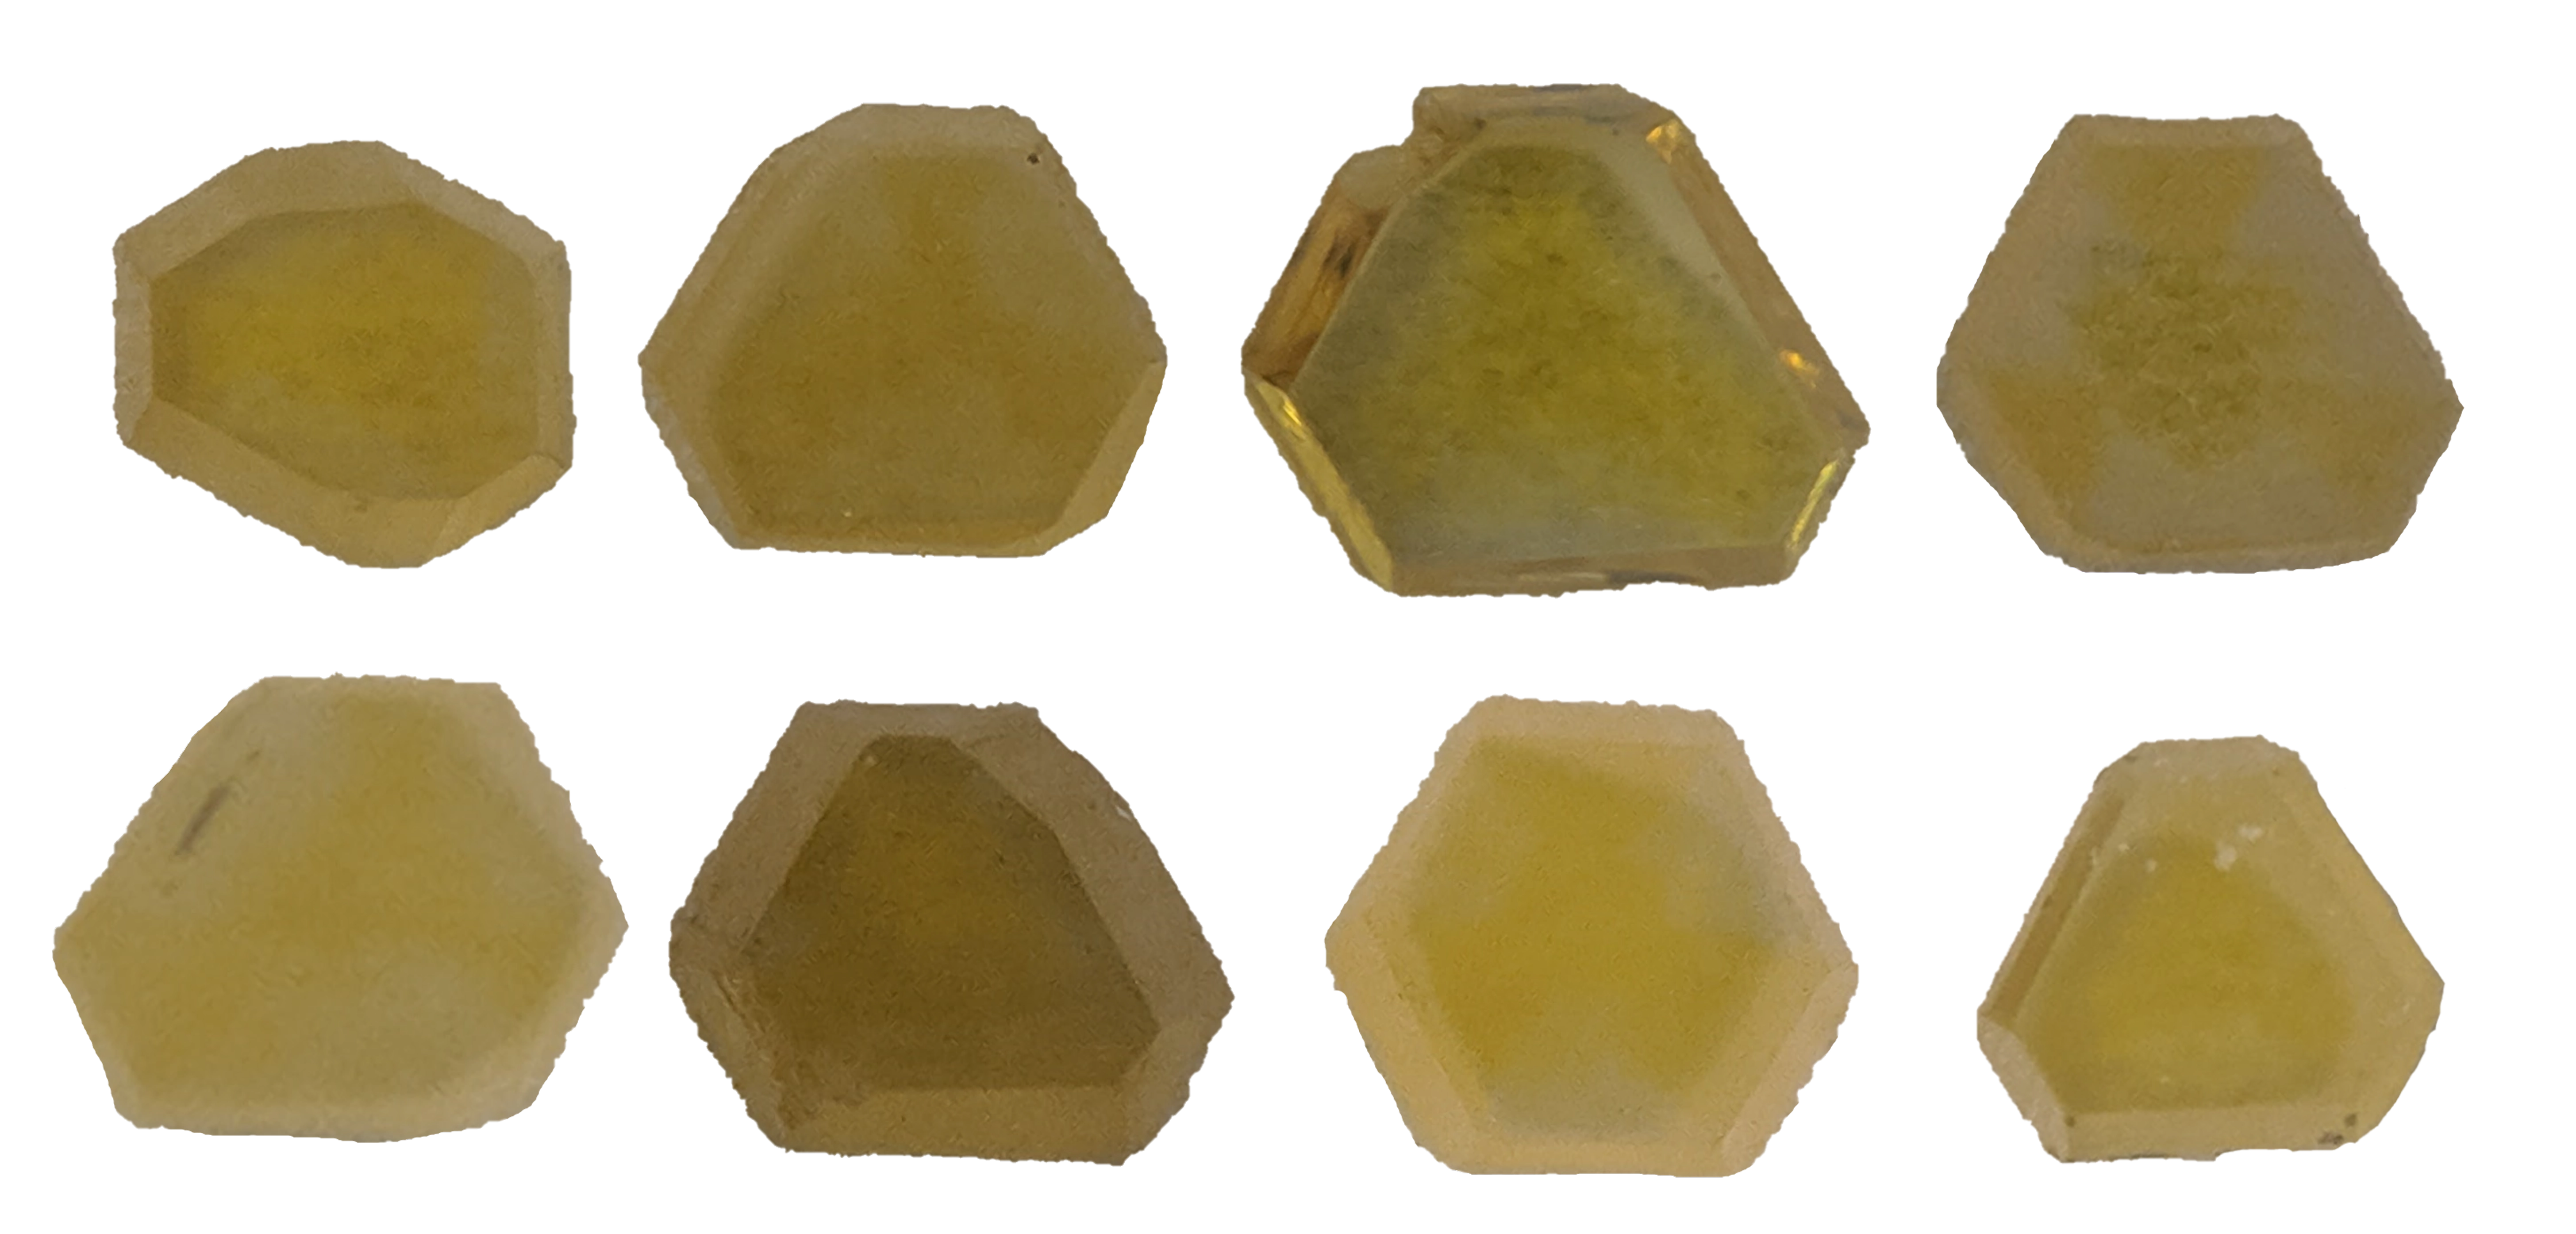
\includegraphics[width=\textwidth]{samples from 2019 - upscaled.png}
\caption{HPHT (111) samples as provided by Element Six, prior to cleaning and deposition.}
\label{fig:111_samples}
\end{figure}

Modern techniques have predominantly converged around variations of dual or tri-acid treatments. \cite{koizumi2000, teraji2000,teraji2003}, and \cite{kociniewski2006, kociniewski2007}, for instance, have favoured a triacid mix of \ce{H2SO4}:\ce{HNO3}:\ce{HClO4}, albeit at different ratios and durations. Some researchers such as \cite{kato2005,kato2009} and \cite{suzuki2004}, however, have leaned towards dual acid organic cleans, utilising \ce{H2SO4} and \ce{H2O2} or \ce{H2SO4} and \ce{HNO3}. 

The various methods of surface preparation underscores the importance of optimising cleaning conditions to the specifics of the application in question. Evince technology employed the following standard surface preparation, with a strong focus on ensuring the removal of graphitic carbon and the formation of a consistent oxygen surface termination prior to phosphorous doped CVD growth, and as such this was used for the work in this project:

\paragraph{Decon90/ Deionised (DI) Water - 5 minutes.}
This acts as an initial cleaning step to remove gross contamination, including organic and inorganic residues. It provides a good general cleaning step that removes common contaminants from the sample surface, especially with a sonication bath providing agitation of the submersed samples. 

\paragraph{DI Rinse and Sonication - 5 minutes.}
Rinsing the samples with deionised water and sonicating them to ensure complete removal of the initial Decon90 solution, along with any remaining contaminants. Thorough rinsing is crucial to prevent any residues from the first cleaning step, which might interfere with subsequent processes, especially the chemical reactions in the following cleaning stages.

\paragraph{1:1 \ce{H2SO4} and \ce{H2O2} Mix - 25 minutes at 175\si{\degreeCelsius}.}
This step employs a"piranha solution, a mixture of \ce{H2SO4} and \ce{H2O2}, to further remove organic residues and contaminants. The strong oxidising nature of this mix at the specified temperature ensures the decomposition of most organic matter, preparing the surface for subsequent treatments. The 1:1 ratio was chosen by Evince technology and was in use as their standard operational cleaning step.

\paragraph{DI Rinse and Sonication - 5 minutes.}
A rinsing and sonication step with deionised water is essential to remove any remaining traces of the piranha solution, ensuring that no residues are left that could interfere with the following stages of surface preparation. The use of sonication aids in dislodging any stubborn contaminants that might remain adhered to the surface after the strong acid treatment.

\paragraph{Plasma Asher - 0.6 mbar, 5\% O2 in He mix for 120 seconds.}
This stage utilises a plasma asher to further clean the surface by removing any remaining organic contaminants and surface residues. The plasma, formed from a 5\% O in He mix at a pressure of 0.67 mbar, generates reactive species that etch away impurities from the surface. This prepares the surface for subsequent treatments, ensuring a consistent and clean base for metal deposition or phosphorous growth. The use of helium in the mix helps in controlling the etching rate by reducing the concentration of oxygen that reacts with the surface, ensuring a gentle but effective cleaning process.

\paragraph{Triacid Mix (1:3:4 \ce{HClO4}:\ce{H2SO4}:\ce{HNO3}) - 7 minutes at 230\si{\degreeCelsius}.}
A triacid mixture serves multiple roles in the cleaning process. It primarily oxidises the diamond surface, preparing it for subsequent metal deposition, and ensures the elimination of any graphitic material. Notably, the 3:4:1 ratio was chosen to optimise both oxidation and impurity removal, standing in slight contrast to other literature findings. 

\paragraph{DI Rinse and Sonication (Repeated 3 Times)}
After the particularly strong triacid treatment, it is essential to ensure no residual acids remain on the diamond surface. As such, a thorough DI sonication rinsing step is performed to conclude the surface cleaning process.

\section{Conventional Ohmic Contacts}
Initial work focused on characterising the properties of ohmic contacts to heavily phosphorous doped diamond as grown by Evince technology. Active carriers within phosphorous doped diamond have been studied in the literature intensively via Hall effect measurements, with the dependence of carrier mobility due to different scattering mechanisms being examined experimentally and theoretically for a wide range of dopant concentrations in the \hkl{111} \cite{stenger2013}, \hkl{100} \cite{stenger2021} and \hkl{113} \cite{pinault2021} orientations.

\subsection{Growth of Heavily Phosphorous-Doped Diamond}
The concentration of phosphorus in diamond films can be modulated by adjusting the ratio of phosphorus to the carbon source (typically methane) in the gas phase during deposition. Numerous studies have observed that an increase in this ratio often leads to a corresponding increase in the as grown diamond films phosphorus concentration \cite{ohtani2014, grotjohn2014, kato2007, kato2005, kociniewski2006, temahuki2017, katamune2023, koizumi1997, kato2009}. 
The studies included in this analysis for comparison to films grown by Evince technology predominantly employed samples with a (111) orientation, with the exception of \cite{kato2007}, which focused on (001) oriented samples. The choice of crystal orientation has implications for the growth rate, dopant concentration and effective carrier compensation, which all complicate the analysis \cite{tokuda2016, mortet2022, pinault2021, stenger2021}.

\subsubsection{SIMS Analysis}
Secondary ion mass spectroscopy (SIMS) was performed on two samples to verify that the chosen growth conditions resulted in a highly doped phosphorous doped diamond film. This analysis was performed by Loughborough Surface Analysis Limited (LSA Ltd), with the results for samples A and B depicted in Figures \ref{fig:sims_A} and \ref{fig:sims_B}. During SIMS analysis, LSA began monitoring with the minor carbon isotope, \ce{^{13}C}, and phosphorus. This choice allowed for a high instrument transmission, enabling the detection of low levels of phosphorus while maintaining the \ce{^{13}C} signal on the detector. Upon reaching the substrate, the \ce{^{13}C} signal noticeably decreased. This decrease prompted a shift to a lower instrument transmission and the additional monitoring of \ce{^{12}C}.

Throughout the profile, the \ce{^{12}C} signal remained consistent in both the layer and the substrate. By comparing the ratios of \ce{^{12}C} and \ce{^{13}C} to each other, it was observed that, while the ratio in the substrate aligned with the expected ratio for carbon, the \ce{^{13}C} signal was proportionally stronger in the epilayer. This discrepancy suggests a significant presence of hydrogen in the epilayer, which appears to combine with \ce{^{12}C}, resulting in an overall higher \ce{^{13}C} signal.

\begin{figure}[H]
\centering
\includegraphics[width=\textwidth]{SIMS Depth Profile 49A.png}
\caption{The measured concentration of phosphorous in the grown film as measured via SIMS for sample A.}
\label{fig:sims_A}
\end{figure}

Figure \ref{fig:sims_A} represents the first example of SIMS performed to measure the concentration of phosphorous within the grown phosphorous doped surface layers. This growth layer presents a reasonably consistent profile throughout the first 0.2~\si{\micro\metre}, tailing off towards the maximum thickness of 0.3~\si{\micro\metre}. This demonstrates a high concentration for the majority of the surface layer, as needed for generation of bulk-like n-type material.

\begin{figure}[H]
\centering
\includegraphics[width=\textwidth]{SIMS Depth Profile 63A.png}
\caption{The measured concentration of phosphorous in the grown film as measured via SIMS for sample B.}
\label{fig:sims_B}
\end{figure}

In figure \ref{fig:sims_B}, the second example of SIMS, for another sample, is presented. In contrast to the first sample in figure \ref{fig:sims_A}, this growth layer appears to be very slightly thicker, with a high phosphorous concentration until past 0.3~\si{\micro\metre}. There is also a conspicuous peak at the end of the highly phosphorous doped surface layer, which may represent a higher uptake of phosphorous doping incorporation at the interface between substrate and the highly doped growth layer. It may also be a result of accumulating phosphorous during the depth profiling process itself, and hence could be considered as a physical error, intrinsic to the SIMS depth profiling. A final point regarding the depth profiling process itself is that these depths represent a one hour growth duration, and were used as growth rate estimators. The exact depth may differ slightly from that indicated in these figures, as the precise calibration of this experimental process is unknown, and depth resolution can vary from sample to sample \cite{Fiori2014}. Preferential sputtering, beam uniformity, sample charging and beam or residual gas contamination can all strongly affect the secondary ion signal \cite{Zinner1980}, so it is important to consider the possible variance that may be present in these presented depths.

\subsection{Phosphorous Incorporation}
\begin{figure}[H]
\centering
\includegraphics[width=\textwidth]{grown concentration vs gas ratio.png}
\caption{Phosphorus concentration (\si{\atoms\per\centi\metre\cubed}) of films as a function of measured [P]/[C] ratio. Each marker represents a different study, with scatter points indicating separate samples. The solid lines represent theoretical phosphorus concentrations for given efficiencies of phosphorus incorporation into the lattice. \cite{ohtani2014,grotjohn2014,kato2007,kato2005, kociniewski2006, temahuki2017, katamune2023, koizumi1997, kato2009}}
\label{fig:phos_concentration}
\end{figure}
Figure \ref{fig:phos_concentration} shows the efficiency of phosphorous incorporation from the gas phase into the resulting doped diamond lattice across various ratios. Theoretical efficiencies of incorporation, ranging from 100\% to 0.1\%, are represented as solid lines. The theoretical efficiency of incorporation for phosphorus from the gas phase into the resulting diamond lattice can be considered as:
\begin{equation}
\label{eq:incorporation_breakdown}
    \text{Incorporation efficiency} = \frac{\text{Resulting dopant concentration}}{\text{Dopant:carbon in CVD feed-gas} \times \text{Atomic density of diamond}}
\end{equation}

For futher review of the different incorporation efficiencies as observed in the literature and how CVD growth has been optimised to improve this, please see section \ref{subsection:incorporation_efficiency}. In figure \ref{fig:phos_concentration} the phosphorous doped films as grown by Evince technology in 2021 and 2022 can be seen in the upper portion of P/C ratio growth, with both a relatively high ratio of 5\% phosphine in the methane feed-gas and a similarly high resultant diamond dopant concentration. This dopant concentration has been measured with SIMS in figures \ref{fig:sims_A}, \ref{fig:sims_B} and appears to match that of the literature comparisons.

While figure \ref{fig:phos_concentration} does show a clear correlation of higher film concentrations with a higher ratio of phosphorous in the carbon containing gas phase, there is a limit at which this trend plateaus. The phosphorous concentration appears to reach saturation at around $10^{20}$ atoms/cm$^{3}$, which can be attributed to the limited solubility of phosphorous within the diamond lattice \cite{Koizumi2008-ig}. The phosphorous grown films from Evince appear to be at this saturation limit, with around $1\times10^{20}$ \si{\atoms\per\centi\metre\cubed} of phosphorous detected via SIMS to the $\sim1.76\times10^{23}$ \si{\atoms\per\centi\metre\cubed} of carbon within the diamond lattice.

The wide range of scatter points visible at specific P/C ratios suggests that factors beyond the P/C ratio, such as temperature, pressure, and plasma conditions (particularly in microwave plasma CVD growth), significantly influence the phosphorus concentration within grown films \cite{Lloret2023}.

Furthermore, it suggests that the efficiency of phosphorus incorporation can vary between different growth techniques and experimental setups. The natural tendency for incorporation efficiency to diminish when higher concentrations of phosphorous are present in the gas phase could also be influenced by more than just solubility limitations. Factors such as changes in the plasma conditions, or the formation of phosphorous clusters which are not possible to incorporate into the diamond lattice, may also play a role \cite{Janssen2014}.

In comparison to conventional semiconductor dopants, diamond has remarkably high activation energies. Hence, the ionisation of such deep dopants must be considered fully in any diamond device that utilises phophosphorous donors.

\subsection{Incomplete Ionisation}
At thermal equilibrium, the electron and hole contributions to current flow across a junction are equivalent, resulting in a constant Fermi level across such a junction. With this condition, the Poisson equation for anisotropic materials, determining the electrostatic potential $\psi$ can be simplified:

\begin{equation}
    \label{eq:poisson_3.10_tesfaye}
\end{equation}
\begin{equation}
    n + N^{-}_{a}=p+N^{+}_{d}
    \label{eq:poisson_simplified_tesfaye}
\end{equation}
where n and p are the electron and hole concentrations respectively, $N^{-}_{a}$ gives the concentration of ionised acceptors and $N^{+}_{d}$ is the concentration of ionised donors. This is then solved with the mass action law:

\begin{equation}
    n\cdot p = n^{2}_{i}
    \label{eq:intrinsic_carriers_3.69_tesfaye}
\end{equation}

where $n_{i}$ is the intrinsice carrier concentration. Then, the equilibrium electron or hole concentration in an n or p-type material respectively is given by:

\begin{equation}
    n=\frac{1}{2}\cdot\left(N^{+}_{d}-N^{-}_{a}+\sqrt{\left(N^{+}_{d}-N^{-}_{a}\right)^{2}-4n^{2}_{i}}\right)
    \label{eq:equilibrium_electron_concentration_3.121_tesfaye}
\end{equation}
\begin{equation}
    p=\frac{1}{2}\cdot\left(N^{-}_{a}-N^{+}_{d}+\sqrt{\left(N^{+}_{d}-N^{-}_{a}\right)^{2}-4n^{2}_{i}}\right)
\end{equation}

The concentration of ionised impurity atoms is given by a steady-state Gibbs distribution as in \cite{tcadmanual2001}:
\begin{equation}
    N^{+}_{d} = \frac{N_{d}}{1+g_{d}\cdot\frac{n}{n_{1}}}
    \label{eq:incomplete_ionisation_donors}
\end{equation}
with: 
\begin{equation}
    n_{1}=N_{c}\cdot\exp{-\frac{E_{c}-E_{d}}{k\cdot T}}
    \label{eq:n_{1}_gibbs_distribution}
\end{equation}
or:
\begin{equation}
    N^{+}_{a} = \frac{N_{a}}{1+g_{a}\cdot\frac{p}{p_{1}}}
    \label{eq:incomplete_ionisation_acceptors}
\end{equation}
with:
\begin{equation}
    p_{1}=N_{v}\cdot\exp{-\frac{E_{a}-E_{v}}{k\cdot T}}
    \label{eq:p_{1}_gibbs_distribution}
\end{equation}

where $N_{d,a}$ are the substitutional and hence active dopant concentrations of donors and acceptors respectively. The ground state degeneracy factor for the donor impurity level in diamond $g_{d} = 2$, since a donor level can accept one electron with either spin, or have no electron at all \cite{koizumi2018:ch2}. The ground state degeneracy factor for acceptor levels is $g_{a}=4$ as each acceptor impurity level can accept a hole of either spin, with a doubly degenerate impurity level as a result of the two degenerate valence bands at $\Vec{k}=0$.

It can also be more convenient to express the ionisation fraction in terms of the carrier concentrations, instead of the relevant quasi-Fermi levels. Taking the Fermi-Dirac statistics form of the carrier concentrations, rather than the Maxwell-Boltzmann form, simply adds the $\gamma_{n,p}$ parameter:

\begin{equation}
    n_{2}=N_{c}\gamma_{n}\cdot\exp{-\frac{E_{c}-E_{f}}{k\cdot T}}
    \label{eq:n_{2}_fermi_distribution}
\end{equation}

\begin{equation}
    p_{2}=N_{c}\gamma_{p}\cdot\exp{-\frac{E_{fp}-E_{v}}{k\cdot T}}
    \label{eq:p_{2}__fermi_distribution}
\end{equation}

In the non-degenerate limit, the Fermi-Dirac distribution gives the Maxwell-Boltzmann distribution and $\gamma_{n,p}=1$. This can be used to define the relevant quasi-Fermi levels as:

\begin{equation}
    E_{fn} = kT\ln{\frac{n}{\gamma_{n}N_{c}}}+E_{c}
    \label{eq:quasi-fermi_levels_carriers_n}
\end{equation}

\begin{equation}
    E_{fp} = -kT\ln{\frac{n}{\gamma_{p}N_{v}}}+E_{v}
    \label{eq:quasi-fermi_levels_carriers_p}
\end{equation}

with the resulting fraction of ionised carriers given in the form:

\begin{equation}
    \frac{N_{d}^{+}}{N_{d}} = \frac{1}{1+\frac{g_{d}n}{\gamma_{n}N_{c}}\exp{\frac{\Delta E_{d}}{kT}}}
    \label{eq:incomplete_ionisation_final_n}
\end{equation}

\begin{equation}
    \frac{N_{a}^{+}}{N_{a}} = \frac{1}{1+\frac{g_{a}p}{\gamma_{p}N_{v}}\exp{\frac{\Delta E_{a}}{kT}}}
    \label{eq:incomplete_ionisation_final_p}
\end{equation}

\begin{figure}[h]
    \centering
    \includegraphics[width=0.97\textwidth]{active_carriers.png}
    \caption{The number of active carriers according to the thermal ionisation equation with a donor energy level of 0.6 \si{\electronvolt}}
    \label{fig:active_carriers}
\end{figure}

where $\Delta E_{d}=E_{c}-E_{d}$ and $\Delta E_{a}=E_{a}-E_{v}$. The results of this equation for phosphorous are shown in figure \ref{fig:active_carriers}. At room temperature with a phosphorous concentration of $1\times10^{20}$ \si{\per\centi\metre\cubed}, the active carrier concentration can be as low as $5.25\times10^{9}$ \si{\per\centi\metre\cubed}, or $5.25\times10^{-9}\%$ which is also demonstrated in other works with hall effect measurements. At 300\si{\degreeCelsius} this is raised to an active carrier concentration of $5.30\times10^{14}$ \si{\per\centi\metre\cubed}, or $5.30\times10^{-4}\%$ of the doping concentration. Hence, this will be a significant factor in the sheet resistance of phosphorous doped diamond. 

\subsubsection{Partly compensated donors}
Along with the thermal ionisation of donors, it is also important to consider the compensation of donors within diamond. The effective carrier concentration, taking into account the presence of compensating acceptor states, can be given with the following equation:
\begin{equation}
    \frac{n\left(N_{A}+n\right)}{N_{D}-N_{A}-n} = \frac{N_{C}}{g_{d}}\exp{-\frac{E_{d}}{kT}}
    \label{eq:carrier_compensation_koizumi2018}
\end{equation}
where $N_{D,A}$ are the carrier concentrations, $k$ is the Boltzmann constant, $T$ is the temperature and $N_{C}$ is the effective density of state, expressed in this case as:
\begin{equation}
    N_{C} = 12\left(\frac{2\pi m^{*}_{e}kT}{h^{2}}\right)^{3/2}
    \label{eq:carrier_compensation_density_of_state}
\end{equation}
where the effective mass of donor electrons $m^{*} = 0.55m_{e}$ ($m_{e}$) is the mass of a free electron) and $h$ is the Planck constant.
\subsection{Ti/Pt/Au Contacts}
\begin{table}[h]
\centering
\caption{A summary of relevant samples for this subsection.}
\label{table:short_samples_summary}
\begin{tabular}{|c|c|c|c|c|}
\hline
Sample & Batch & Thickness (\si{\micro\metre}) & Contacts & Characterisation \\
\hline
A & 1 & 0.3 & None & SIMS \\
B & 1 & 0.3 & None & SIMS \\
C & 2 & 0.3 & Ti/Pt/Au - 850\si{\degreeCelsius} 30 mins  & TLM, AFM \\
D & 2 & 0.3 & Ti/Pt/Au - 600\si{\degreeCelsius} 300 mins & TLM, AFM \\
% Add more samples here
\hline
\end{tabular}
\end{table}
Two samples (C and D) were used for initial TLM characterisation. With the same growth conditions as for samples A and B, a heavily phosphorous doped surface layer was grown via MPCVD following the standard cleaning process. In figure \ref{fig:TLMB} the final Ti/Pt/Au structure used for both is shown. The linear TLM structure can be seen on the lower portion of the sample's surface. When compared, the sample dimensions were comparable, with sizes of $3.7\times3.8$ \si{\milli\metre} for sample C and $3.9\times4.1$ \si{\milli\metre} for sample D. The Ti/Pt/Au contacts used were fabricated via electron-beam lithography, with nominal thicknesses of 20/20/100 \si{\micro\metre} respectively. Sample C was annealed at 850\si{\degreeCelsius} for 30 minutes, while sample D was annealed at 600\si{\degreeCelsius} for 300 minutes, as summarised in table \ref{table:short_samples_summary}. Annealing conditions were chosen such that a shorter, high temperature anneal could be compared to a longer, low temperature anneal. Crucial to the success of such annealing is the formation of TiC at the diamond interface \cite{teraji2000, teraji2003}, which is examined further in section \ref{subsubsec:annealing}, but generally is observed from temperatures as low as $400$ \si{\degreeCelsius}. This is explored further in section \ref{subsubsec:annealing_rationale}, for further device fabrication.

The surface thicknesses for samples C and D are estimated at 0.3 \si{\micro\metre}, as while grown in different batches, the duration of phosphorous growth was consistent between batch 1 and 2, hence the SIMS data for samples A and B may be considered representative for these subsequent samples.

\begin{figure}[ht]
\centering
\includegraphics[width=0.6\textwidth]{Chapter3/Figs/Raster/Sample D 2019/TLMB.jpg}
\caption{Sample B with linear TLM contacts, as seen with an optical microscope.}
\label{fig:TLMB}
\end{figure}

\section{Linear Transfer Length Method (TLM) and Richardson Analysis}
In this section, the analysis of I-V curves for samples C and D ranging from room temperature to 300\si{\degreeCelsius} are presented. Due to the phosphorous donor ionisation energy of around 0.6~\si{\electronvolt}, there is a very significant temperature dependence. At room temperature, the smallest channel width of approximately 3.5~\si{\micro\metre} drew a current density of approximately $1.57\times10^{-6}$~\si{\ampere\per\centi\metre\squared} with a potential bias of 10 \si{\volt}, while at 300\si{\degreeCelsius} this increased to $1.08\times10^{-4}$\si{\ampere\per\centi\metre\squared}. 

\subsection{Ti/Pt/Au I-V Results}
\label{subsec:iv_results_ltlm_tiptau}
The linear plots of measured current vs applied voltage for samples C and D over temperatures of 21, 150 and 300 \si{\degreeCelsius} are presented in this section, for a bias range of $\pm10$ \si{\volt}.
\begin{figure}[H]
    \centering
    \includegraphics[width=0.97\textwidth]{Chapter3/Figs/Raster/1V IV characteristics at 21 C.png}
    \caption{A linear plot of the measured current against applied voltage for three channel lengths, $\pm1$ \si{\volt}, at 21\si{\degreeCelsius} (sample C).}
    \label{fig:1V_C_current_voltage_21}
\end{figure}
For reference, a limited bias range of $\pm1$ \si{\volt} is plotted in figure \ref{fig:1V_C_current_voltage_21} without error bars to examine the potential magnitudes of error. Typical errors for the B1500A are typically no higher than 2 \si{\pico\ampere} as calibrated, with the measured data hence only showing noise when the applied bias is very close to 0 \si{\volt}. As the equipment error of 2~\si{\pico\ampere} is considered to be the ideal calibrated error, an increased worst case error of 5~\si{\pico\ampere} is used for IV plots to account for the sinusoidal noise of approximate amplitude of 5~\si{\pico\ampere} observed in figure \ref{fig:1V_C_current_voltage_21}.

\begin{figure}[H]
    \centering
    \includegraphics[width=\textwidth]{Chapter3/Figs/Raster/Sample C 2019/IV/10V IV characteristics at 21 C.jpg}
    \caption{A linear plot of the measured current against applied voltage for all channel lengths at 21\si{\degreeCelsius} (sample C).}
    \label{fig:C_current_voltage_21}
\end{figure}
Figure \ref{fig:C_current_voltage_21} shows the room temperature IV characteristics of sample C across all LTLM channels. The current drawn here reflects a large sheet resistance and contact resistance to the highly phosphorous doped diamond
\begin{figure}[H]
    \centering
    \includegraphics[width=\textwidth]{Chapter3/Figs/Raster/Sample D 2019/IV/10V IV characteristics at 21 C.jpg}
    \caption{A linear plot of the measured current against applied voltage for all channel lengths at 21\si{\degreeCelsius} (sample D).}
    \label{fig:D_current_voltage_21_10V}
\end{figure}
Figure \ref{fig:D_current_voltage_21_10V} shows the room temperature IV characteristics of sample D across all LTLM channels. Again the high sheet resistance produces a current of~\si{\pico\ampere}, though this sample has a slightly narrower smallest channel size of 2.8~\si{\micro\metre}.
\begin{figure}[H]
    \centering
    \includegraphics[width=\textwidth]{Chapter3/Figs/Raster/Sample C 2019/IV/10V IV characteristics at 150 C.jpg}
    \caption{A linear plot of the measured current against applied voltage for all channel lengths at 150\si{\degreeCelsius} (sample C).}
    \label{fig:C_current_voltage_150}
\end{figure}
In figure \ref{fig:C_current_voltage_150} the IV characteristics of sample C at 150\si{\degreeCelsius} show a reduced resistance to that of the room temperature case. While the current is still low overall, this is a good indicator of a semiconducting channel.
\begin{figure}[H]
    \centering
    \includegraphics[width=\textwidth]{Chapter3/Figs/Raster/Sample D 2019/IV/10V IV characteristics at 150 C.jpg}
    \caption{A linear plot of the measured current against applied voltage for all channel lengths at 150\si{\degreeCelsius} (sample D).}
    \label{fig:D_current_voltage_150_10V}
\end{figure}
Similarly to sample C, figure \ref{fig:D_current_voltage_150_10V} shows that sample D has an IV characteristic that follows the same trend for higher temperatures.
\begin{figure}[H]
    \centering
    \includegraphics[width=\textwidth]{Chapter3/Figs/Raster/Sample C 2019/IV/10V IV characteristics at 300 C.jpg}
    \caption{A linear plot of the measured current against applied voltage for all channel lengths at 300\si{\degreeCelsius} (sample C).}
    \label{fig:C_current_voltage_300}
\end{figure}
Figure \ref{fig:C_current_voltage_300} represents the highest temperature tested for sample C at 300~\si{\degreeCelsius}. The current is still very low in this potential bias range, and so the linear appearance of this data may be deceptive.
\begin{figure}[H]
    \centering
    \includegraphics[width=\textwidth]{Chapter3/Figs/Raster/Sample D 2019/IV/10V IV characteristics at 300 C.jpg}
    \caption{A linear plot of the measured current against applied voltage for all channel lengths at 300\si{\degreeCelsius} (sample D).}
    \label{fig:D_current_voltage_300_10V}
\end{figure}
Figure \ref{fig:D_current_voltage_300_10V} shows the highest temperature of 300\si{\degreeCelsius} for sample D. Despite being comparable to sample C, the lower channel spacing for this sample consistently shows a less linear behaviour, hinting at a Schottky behaviour for higher potential biases. To investigate this further, higher potential bias ranges were performed for sample D. Unfortunately the same bias ranges were not performed for sample C. Included here, for comparison, are the 50~\si{\volt} IV data for sample D at room temperature and 300~\si{\degreeCelsius}.

\begin{figure}[H]
    \centering
    \includegraphics[width=\textwidth]{Chapter3/Figs/Raster/Sample D 2019/IV/50V IV characteristics at 21 C.png}
    \caption{A linear plot of the measured current against applied voltage for all channel lengths at 21\si{\degreeCelsius} (sample D).}
    \label{fig:D_current_voltage_21_50V}
\end{figure}
Figure \ref{fig:D_current_voltage_21_50V} shows the room temperature IV characteristics of sample D for the potential bias range of $\pm50$~\si{\volt}. It is immediately apparent that the linear plots of lower potential biases becomes a Schottky-appearing trend for all channels at higher potential biases. This is despite the contacts in use here being that of conventionally "Ohmic" forming metals (Ti/Pt/Au), with annealing and a high concentration of phosphorus doping in the diamond surface layer.

\begin{figure}[H]
    \centering
    \includegraphics[width=\textwidth]{Chapter3/Figs/Raster/Sample D 2019/IV/50V IV characteristics at 300 C.png}
    \caption{A linear plot of the measured current against applied voltage for all channel lengths at 300\si{\degreeCelsius} (sample D).}
    \label{fig:D_current_voltage_300_50V}
\end{figure}
Figure \ref{fig:D_current_voltage_300_50V} provides the highest temperature IV data for the bias range of $\pm50$~\si{\volt} for sample D. This continues the trend of lower measured resistances at higher temperatures, with the addtional context of higher potential biases revealing a Schottky behaviour for these annealed Ti/Pt/Au contacts.

\subsection{Ti/Pt/Au J-V Results}
This section presents the current density vs applied voltage plots for samples C and D at temperatures of 21, 150, and 300\si{\degreeCelsius}. The bias range used is $\pm10$ \si{\volt}. Error bars representing a current error of $1$ \si{\pico\ampere}, are included in all plots. Data points have been processed using a running average over three consecutive points. 

\begin{figure}[h]
    \centering
    \includegraphics[width=0.97\textwidth]{Sample C 2019/10V_Current_Density_vs_Voltage_Temperature_21_log.png}
    \caption{A log-linear plot of the measured current density against applied voltage for all channel lengths at 21\si{\degreeCelsius} (sample C).}
    \label{fig:10V_current_density_21_C}
\end{figure}
\begin{figure}[h]
    \centering
    \includegraphics[width=0.97\textwidth]{Sample D 2019/10V_Current_Density_vs_Voltage_Temperature_21_log.png}
    \caption{A log-linear plot of the measured current density against applied voltage for all channel lengths at 21\si{\degreeCelsius} (sample D).}
    \label{fig:10V__current_density_21_D}
\end{figure}

\begin{figure}[h]
    \centering
    \includegraphics[width=0.97\textwidth]{Sample C 2019/10V_Current_Density_vs_Voltage_Temperature_250_log.png}
    \caption{A log-linear plot of the measured current density against applied voltage for all channel lengths at 150\si{\degreeCelsius} (sample C).}
    \label{fig:10V_current_density_150_C}
\end{figure}
\begin{figure}[h]
    \centering
    \includegraphics[width=0.97\textwidth]{Sample D 2019/10V_Current_Density_vs_Voltage_Temperature_250_log.png}
    \caption{A log-linear plot of the measured current density against applied voltage for all channel lengths at 150\si{\degreeCelsius} (sample D).}
    \label{fig:10V__B_current_density_150_D}
\end{figure}

\begin{figure}[h]
    \centering
    \includegraphics[width=0.97\textwidth]{Sample C 2019/10V_Current_Density_vs_Voltage_Temperature_300_log.png}
    \caption{A log-linear plot of the measured current density against applied voltage for all channel lengths at 300\si{\degreeCelsius} (sample C).}
    \label{fig:10V_current_density_300_C}
\end{figure}
\begin{figure}[h]
    \centering
    \includegraphics[width=0.97\textwidth]{Sample D 2019/10V_Current_Density_vs_Voltage_Temperature_300_log.png}
    \caption{A log-linear plot of the measured current density against applied voltage for all channel lengths at 300\si{\degreeCelsius} (sample D).}
    \label{fig:10V_current_density_300_D}
\end{figure}

\FloatBarrier

\subsubsection{Analysis of J-V Data}
In figures \ref{fig:10V_current_density_21_C}--\ref{fig:10V_current_density_300_D}, the measured current characteristics as converted into current density measurements are plotted. While most of these plots are quite natural given the prior IV figures, figure \ref{fig:10V_current_density_300_D} in particular is noteworthy due to the off centre dataset for the largest channel size. During high-temperature testing of sample D, the electrical characteristics indicated a significant short in the system. Upon investigation, it was discovered that a large flake of the deposited metal had detached from the diamond surface and come into contact with one of the electrical probes during the test procedure. Consultations with Evince Technology indicated that poor adhesion may be a common problem when annealing times significantly exceed 30 minutes. Therefore, the electrical data presented here is that which was measured prior to the flake delamination. The off centre data of figure \ref{fig:10V_current_density_300_D} indicates a large error in the system, which is highly likely to be the onset of issues due to delamination. 

Otherwise, these current density plots show a few clear trends, such as sample D consistently showing higher current densities than sample C across the $\pm10$~\si{\volt} range. Both samples generally show a clear dependence of the measured current density on the channel widths, indicating higher resistances for increased channel lengths, and the samples show a clear increase of measured current as a function of the temperature, indicating the reduction of resistance via ionisation of deep donors as predicted for phosphorous doped diamond. The same trends can be seen in the linear I-V plots from the previous section. The highest temperature $\pm50$~\si{\volt} JV plot of sample D is included for a final comparison with the higher voltage region. Note that in all current density plots, error bars are plotted as calculated from the error on current measurements, previously described in section \ref{subsec:iv_results_ltlm_tiptau}. They are most visible in the low voltage, low current density regions, and highlight the difficulty in interpreting very low voltages for these devices.

\begin{figure}[H]
    \centering
    \includegraphics[width=0.97\textwidth]{Sample D 2019/50V_Current_Density_vs_Voltage_Temperature_300_log.png}
    \caption{A log-linear plot of the measured current density against applied voltage for all channel lengths at 300\si{\degreeCelsius} (sample D).}
    \label{fig:50V_current_density_300_D}
\end{figure}

Figure \ref{fig:50V_current_density_300_D} shows this final comparison of J-V data for a $\pm50$~\si{\volt} range. The slight offset in the highest channel length indicating a delamination error is difficult to pick out at this scale, with no other significant trends visible at the higher voltage range. Generally, this represents a double Schottky behaviour well.

\subsection{Richardson Plots}
The operating current for an ideal Schottky diode under a forward bias where $qV > 3kT$, based on the thermionic emission of electrons, is given by \cite{sze2006} as:
\begin{equation}
    I=I_{s}\exp{qV/nkT}\left[1-\exp{-qV/kT}\right]
\end{equation}
Where $I_{s}$ is the saturation current, $q$ is the elementary charge, $V$ is the applied voltage, $n$ is the diode ideality factor, $k$ is the Boltzmann constant and $T$ is the temperature. In this ideal case, the carrier conduction in a forward bias is dominated by the thermal emission of carriers from the semiconductor over a spatially homogenous barrier into the metal. This equation can be rearranged into a format that allows for linear analysis:

\begin{equation}
    \ln{\frac{I}{1-\exp{\left(-\beta V\right)}}} = \frac{\beta V}{n} + \ln{I_{s}}
    \label{eq:thermionic_emission_graphical}
\end{equation}

Here, \(\beta=\frac{q}{kT}\). The saturation current $I_{s}$ is given by:

\begin{equation}
\label{eq:richarson-linear}
    \ln{\frac{I_{s}}{AT^{2}}} = -q\frac{\phi_{Beff}}{kT} + \ln{A^{*}_{eff}}
\end{equation}

Where $A^{*}_{eff}$ is the effective Richardson constant, $A$ is the area of the Schottky contact and $\phi_{Beff}$ is the effective barrier height. The Richardson constant, \( A^{*} \), which characterises the thermionic emission process, arises from the Richardson-Dushman equation for thermionic emission \cite{sze2006}.

In practice, \( A \) can vary for different materials. For instance, in polycrystalline metals, \( A \) can range from about \SI{32}{\ampere\per\centi\meter\squared\per\kelvin\squared} to \SI{160}{\ampere\per\centi\meter\squared\per\kelvin\squared} and can vary even more widely for oxide and composite surfaces. The theoretical value of the Richardson constant is given by:
\begin{equation}
    A^{*} = \frac{4\pi qk^{2}m^{*}}{h^{3}}
\end{equation}
where \(m^{*}\) is the effective electron mass and \(h\) is Planck's constant. The effective electron masses within phosphorous doped diamond are taken to be $m_{\perp}=0.306m_{0}$ and $m_{\parallel}=1.81m_{0}$, from Gheeraert et al. \cite{Gheeraert2001} who determined the masses via infrared absorption spectroscopy of phosphorous doped films. For further discussion on the background of the effective electron masses in phosphorous doped diamond, see section \ref{subsubsec:effective_electron_masses_in_phosphorous_doped_diamond}.

\begin{figure}[h]
    \centering
    \includegraphics[width=\textwidth]{Chapter3/Figs/Raster/Sample C 2019/newRichardson_Plot_10V.png}
    \caption{A conventional Richardson plot for the various channel widths tested (Sample C, 10V range).}
    \label{fig:richardsonC}
\end{figure}

\begin{table}[h]
    \centering
    \begin{tabular}{|c|c|c|c|}
        \hline
        Channel (\si{\micro\metre}) & Barrier (\si{\electronvolt}) & $A*_{eff}$ (\si{\ampere\per\centi\metre\squared\per\kelvin\squared}) & $R^{2}$\\ \hline
        3.529 & 0.1515  & 3.92e-09 &0.9888 \\ 
        5.064 & 0.1565  & 3.12e-09 &0.9892 \\ 
        6.949 & 0.1576  & 2.46e-09 &0.9884 \\ 
        8.947 & 0.1599  & 2.07e-09 &0.9918 \\ 
        10.720 & 0.1595  & 1.73e-09 &0.9865 \\ 
        12.890 & 0.1709 & 2.29e-09 &0.9889 \\ 
        14.930 & 0.1669  & 1.73e-09 &0.9876 \\ 
        16.970 & 0.1615  & 1.15e-09 &0.9900 \\ 
        \hline
    \end{tabular}
    \caption{Extracted parameters from the Richardson plot for sample C at 10~\si{\volt}.}
    \label{tab:richardsonC}
\end{table}

\begin{figure}
    \centering
    \includegraphics{Chapter3/Figs/Raster/Sample D 2019/newRichardson_Plot_10V.png}
    \caption{A conventional Richardson plot for the various channel widths tested (Sample D, 10 V range).}
    \label{fig:richardsonD}
\end{figure}

\begin{table}[h]
    \centering
    \begin{tabular}{|c|c|c|c|c|}
        \hline
        Channel (\si{\micro\metre}) & Barrier (\si{\electronvolt})  & $A*_{eff}$ (\si{\ampere\per\centi\metre\squared\per\kelvin\squared}) & $R^{2}$\\ \hline
        2.803 & 0.1639  & 8.08e-09 &0.9799 \\ 
        4.862 & 0.1789 & 2.65e-09 &0.9757 \\ 
        6.945 & 0.1806  & 1.90e-09 &0.9739 \\ 
        9.029 & 0.1809 & 1.46e-09 &0.9725 \\ 
        11.110 & 0.1780  & 1.16e-09 &0.9679 \\ 
        13.150 & 0.1765  & 8.86e-10 &0.9603 \\ 
        15.130 & 0.2272  & 4.11e-09 &0.8324 \\ 
        \hline
    \end{tabular}
    \caption{Extracted parameters from the Richardson plot for sample D at 10~\si{\volt}.}
    \label{tab:richardsonD_10V}
\end{table}

\begin{figure}[h]
    \centering
    \includegraphics[width=\textwidth]{Chapter3/Figs/Raster/Sample D 2019/newRichardson_Plot_50V.png}
    \caption{A conventional Richardson plot for the various channel widths tested (Sample D, 50 V range).}
    \label{fig:richardsonD_50V}
\end{figure}

\begin{table}[h]
    \centering
    \begin{tabular}{|c|c|c|c|}
        \hline
        Channel (\si{\micro\metre}) & Barrier (\si{\electronvolt}) & $A*_{eff}$ (\si{\ampere\per\centi\metre\squared\per\kelvin\squared}) & $R^{2}$\\ \hline
        2.803 & 0.0824  & 3.49e-08 &0.9670 \\ 
        4.862 & 0.1265  & 1.24e-08 &0.9729 \\ 
        6.945 & 0.1425 & 8.95e-09 &0.9731 \\ 
        9.029 & 0.1539 & 7.09e-09 &0.9727 \\ 
        11.110 & 0.1567  & 5.77e-09 &0.9710 \\ 
        13.150 & 0.1681  & 4.86e-09 &0.9651 \\ 
        15.130 & 0.2200 & 2.14e-08 &0.8304 \\ 
        \hline
    \end{tabular}
    \caption{Extracted parameters from the Richardson plot for sample D at 50~\si{\volt}.}
    \label{tab:richardsonD_50V}
\end{table}

To examine the method of electron emission from the contacts, a conventional Richardson plot is shown in figures \ref{fig:richardsonC} and \ref{fig:richardsonD} for a constant bias range of $\pm10$ \si{\volt}. By fitting a linear relationship to these data, as according to equation \ref{eq:thermionic_emission_graphical}, the average Schottky barrier height for samples C and D is extracted to be 0.161~\si{\electronvolt} and 0.150 \si{\electronvolt}, with a standard deviation of $5.56$~\si{\milli\electronvolt} and $38.6$ \si{\milli\electronvolt}, respectively. The exact results determined from the best-fit linear lines are shown in tables \ref{tab:richardsonC} and \ref{tab:richardsonD_10V}.

\begin{figure}[htbp]
    \centering
    \begin{subfigure}[b]{0.49\textwidth}
        \includegraphics[width=\textwidth]{Chapter3/Figs/Raster/barrier_comparison.png}
        \caption{The measured values for the barrier heights as a function of the linear TLM channel length.}
        \label{fig:barrier}
    \end{subfigure}
    \hfill % Spaces the figures a bit
    \begin{subfigure}[b]{0.49\textwidth}
        \includegraphics[width=\textwidth]{Chapter3/Figs/Raster/richardson_comparison.png}
        \caption{The measured values for the Richardson constant as a function of the linear TLM channel length.}
        \label{fig:richardson}
    \end{subfigure}
    \caption{(a) Effective barrier height vs. linear TLM channel length. (b) Effective Richardson constant vs. linear TLM channel length.}
    \label{fig:side_by_side_barrier_richardson}
\end{figure}

 One observation from these data is that sample C displays a relatively constant barrier height, regardless of the channel length, while sample D shows a proportionality between the channel length and the effective barrier height. This could be due to the difference in the smallest channel sizes. While both sets of metal contacts were formed with the same shadow mask in the process of metal deposition via photolithography, the as formed contacts had a measurably different channel length at the smallest scales. The smallest channel measured by AFM in sample C was $\sim3.5$~\si{\micro\metre}, while sample D had a channel length of $\sim2.8$~\si{\micro\metre}. A visual comparison of the barrier heights extracted for both samples, over the full range of channel lengths and for differing potential biases in the case of sample D is provided in figure \ref{fig:barrier}.%incorrect need to replot

 Further analysis is provided by figure \ref{fig:richardsonD_50V} and table \ref{tab:richardsonD_50V}, in which the 50~\si{\volt} measurements as processed in a Richardson plot are summarised. The effective Schottky barrier height as observed in this case is significantly lower than for the 10~\si{\volt} measurements, reducing from $\sim0.150$~\si{\electronvolt} to $\sim0.082$~\si{\electronvolt} for the shortest channel spacing of $\sim2.8$~\si{\micro\metre}. This is most likely due to image force barrier lowering of the Schottky contacts \cite{Schroder2006-sx, sze2006}. This is also a natural consequence of equation \ref{eq:richarson-linear}, as the barrier height is dependent upon the measured current, but the derivation extends from the classical point charge derivation of image force effects for a metal contacting a semiconductor. Section \ref{subsec:image_force_effect_schottky_effect} contains a further exploration of the image force effect and how this reduces the Schottky barrier to thermionic emission for differing electric field strengths.

Additional complexity may be considered as a result of the "low-temperature" nature of the diamond in the temperature range studied here. This may introduce a temperature dependency for the barrier height, which can be written as \cite{Schroder2006-sx}:

 \begin{equation}
     \phi_{B}(T) = \phi_{B}(0) - \xi T
     \label{eq:temp_dependent_barrier}
 \end{equation}
 
where $\xi$ is a proportionality constant. Given the good linear fits overall for the Richardson plots, this is not considered any further, but it remains as a possible complicating factor in these results. 
 
The smallest channel of sample D at 50~\si{\volt} bias presents an effective barrier height of $\sim0.08$ \si{\electronvolt}, while the largest channel was $\sim0.22$ \si{\electronvolt}. Similarly, there is an inverse proportionality between the channel length and the observed Richardson constant for both samples, with sample C's Richardson constant consistently an order of magnitude lower than sample D. This is represented visually in figure \ref{fig:side_by_side_barrier_richardson}, as the relationship between the effective Richardson constant and the channel length for all data is quite complex. 

\subsection{TLM Results}
\begin{figure}[H]
    \centering
    \includegraphics[width=\textwidth]{Chapter3/Figs/Raster/Sample C 2019/TLM/All Lin Reg TLM Plot Linear scale.png}
    \caption{Sample C - the channel spacing vs measured total resistance for all temperatures ($\pm10$ \si{\volt}).}
    \label{fig:c_tlm_lin}
\end{figure}

\begin{figure}[H]
    \centering
    \includegraphics[width=\textwidth]{Chapter3/Figs/Raster/Sample C 2019/TLM/All Lin Reg TLM Plot Log scale.png}
    \caption{Sample C - the channel spacing vs log scale measured total resistance for all temperatures ($\pm10$ \si{\volt}).}
    \label{fig:c_tlm_log}
\end{figure}

\begin{table}[h]
\caption{The summarised extracted parameters via LTLM on sample C for a 10 V range.}
\label{tab:c_ltlmss}
\centering
\begin{tabular}{lllll}
\toprule
T\si{\degreeCelsius} & $R_{sh}$ $(\Omega/\square)$ & $\rho_{s}$ $(\Omega\cdot cm)$ & $\rho_{c}$ $(\Omega\cdot cm^2)$ & R$^2$ \\
\midrule
21 & $1.10\times 10^{+12}$ & $1.32\times 10^{+08}$ & $4.72\times 10^{+05}$ & $9.95\times 10^{-01}$ \\
50 & $6.33\times 10^{+11}$ & $7.60\times 10^{+07}$ & $2.51\times 10^{+05}$ & $9.93\times 10^{-01}$ \\
100 & $2.30\times 10^{+11}$ & $2.76\times 10^{+07}$ & $1.88\times 10^{+05}$ & $9.91\times 10^{-01}$ \\
150 & $9.44\times 10^{+10}$ & $1.13\times 10^{+07}$ & $1.21\times 10^{+05}$ & $9.49\times 10^{-01}$ \\
200 & $4.35\times 10^{+10}$ & $5.22\times 10^{+06}$ & $5.81\times 10^{+04}$ & $9.64\times 10^{-01}$ \\
250 & $2.28\times 10^{+10}$ & $2.74\times 10^{+06}$ & $3.06\times 10^{+04}$ & $9.69\times 10^{-01}$ \\
300 & $1.16\times 10^{+10}$ & $1.39\times 10^{+06}$ & $2.43\times 10^{+04}$ & $9.28\times 10^{-01}$ \\
\bottomrule
\end{tabular}
\end{table}

Table \ref{tab:c_ltlmss} presents the summary of LTLM analysis for sample C. At room temperature, a specific contact resistivity of 472~\si{\kilo\ohm\centi\metre\squared} is observed, reducing to 24.3~\si{\kilo\ohm\centi\metre\squared} at 300\si{\degreeCelsius}. This is paired with a phosphorous doped diamond resistivity ranging from 132~\si{\mega\ohm\centi\metre} to 1.39~\si{\mega\ohm\centi\metre}.

\begin{figure}[H]
    \centering
    \includegraphics[width=\textwidth]{Chapter3/Figs/Raster/Sample D 2019/TLM 10V/All Lin Reg TLM Plot Linear scale.png}
    \caption{Sample D - the channel spacing vs measured total resistance for all temperatures ($\pm10$ \si{\volt}).}
    \label{fig:D_tlm_lin}
\end{figure}

\begin{figure}[H]
    \centering
    \includegraphics[width=\textwidth]{Chapter3/Figs/Raster/Sample D 2019/TLM 10V/All Lin Reg TLM Plot Log scale.png}
    \caption{Sample D - the channel spacing vs log scale measured total resistance for all temperatures ($\pm10$ \si{\volt}).}
    \label{fig:d_tlm_log}
\end{figure}

\begin{table}[h]
\caption{The summarised extracted parameters via LTLM on sample D for a 10 V range.}
\label{tab:d_ltlmss}
\centering
\begin{tabular}{lllll}
\toprule
Temperature\si{\degreeCelsius} & Sheet Resistance $(\Omega/\square)$ & Resistivity $(\Omega\cdot cm)$ & Specific Contact Resistivity $(\Omega\cdot cm^2)$ & R$^2$ \\
\midrule
21 & $4.12\times 10^{+12}$ & $4.94\times 10^{+08}$ & $6.91\times 10^{+06}$ & $9.84\times 10^{-01}$ \\
50 & $2.53\times 10^{+12}$ & $3.04\times 10^{+08}$ & $4.77\times 10^{+06}$ & $9.89\times 10^{-01}$ \\
100 & $9.58\times 10^{+11}$ & $1.15\times 10^{+08}$ & $1.93\times 10^{+06}$ & $9.93\times 10^{-01}$ \\
150 & $3.60\times 10^{+11}$ & $4.32\times 10^{+07}$ & $6.55\times 10^{+05}$ & $9.92\times 10^{-01}$ \\
200 & $1.50\times 10^{+11}$ & $1.81\times 10^{+07}$ & $2.53\times 10^{+05}$ & $9.92\times 10^{-01}$ \\
250 & $6.90\times 10^{+10}$ & $8.28\times 10^{+06}$ & $1.10\times 10^{+05}$ & $9.93\times 10^{-01}$ \\
300 & $2.94\times 10^{+10}$ & $3.53\times 10^{+06}$ & $3.42\times 10^{+04}$ & $9.84\times 10^{-01}$ \\
\bottomrule
\end{tabular}
\end{table}

Table \ref{tab:d_ltlmss} presents the summary of LTLM analysis for sample D. At room temperature, a specific contact resistivity of 6910~\si{\kilo\ohm\centi\metre\squared} is observed, reducing to 34.0~\si{\kilo\ohm\centi\metre\squared} at 300\si{\degreeCelsius}. This is paired with a phosphorous doped diamond resistivity ranging from 132~\si{\mega\ohm\centi\metre} to 1.39~\si{\mega\ohm\centi\metre}.

\subsection{XPS Analysis}
Further to the SIMS analysis of films grown for one hour, X-Ray Photo-electron Spectroscopy (XPS) measurements were performed on a sample that had been used for a four hour deposition of highly phosphorous doped material. This is sample E in table \ref{table:samples_summary}. An additional sample included in this batch of doped diamond growth was then used for circular-TLM measurements. The growth duration was chosen to be 4 hours based on the previous observation via SIMS of a growth rate of 0.3 \si{\micro\metre\per\hour}, with the aim being the production of a $\sim1$ \si{\micro\metre} thick surface layer. This would ensure that any conduction measured through the phosphorous doped diamond film would be comparable to other work in this area, with bulk conduction instead of conduction through nanometre scale material. Note, that for all data presented here, the XPS data comes from just below the sample surface. This is due to an original planned experiment of depth profiling, hence ion beam bombardment was used to etch away the diamond surface and attempt to etch through the phosphorus doped surface layer. However, it was observed that despite a predicted depth of 3~\si{\micro\metre} being reached, no change in the XPS spectra was observed beyond the initial change from surface characterisation and then the cleaned, sub surface characterisation. This was backed up by AFM and attempts to resolve the depth of the etched region via optical profilometry failing to measure any etched region in the diamond surface. Hence, the sub-surface spectra are presented without depth profiling attempted, with the observation from additional characterisation that the "sub-surface" spectra may only represent a clean diamond surface spectra.

\begin{figure}[H]
    \centering
    \includegraphics[width=\textwidth]{Chapter3/Figs/xps_c1s.png}
    \caption{XPS - The C1s scan range.}
    \label{fig:xps_c1s}
\end{figure}

In figure \ref{fig:xps_c1s}, the XPS data taken for the theoretical C1s peak region are shown. Note that the counts per second (CPS) for the peak closely correlating with the sp$^{3}$ C1s 284.8~\si{\electronvolt} peak \cite{Fang2020} is at around $14\times10^{4}$ CPS. The slight side peak visible can be decomposed to reveal that it is centred very closely to the sp$^{2}$ binding energy of 284.2~\si{\electronvolt}, indicating a significant degree of amorphous carbon in the phosphorous doped diamond surface layer \cite{Fang2020}. 

\begin{figure}[H]
    \centering
    \includegraphics[width=\textwidth]{Chapter3/Figs/xps_P2p.png}
    \caption{XPS - The P2p scan range.}
    \label{fig:xps_p2p}
\end{figure}

Figure \ref{fig:xps_p2p} shows the XPS data taken for the binding energy region corresponding to the C-P bond of 132.6~\si{\electronvolt} and the P-O bond of 133.6~\si{\electronvolt} \cite{Yu2019}. While these data are difficult to decompose, the order of magnitude for CPS due to phosphorous bonds can be read as approximately 680 CPS. As the scale of CPS with these datasets is calibrated prior to the measurements being taken, these CPS measurements can be taken as a relative scale of carbon to phosphorous atomic concentrations. There is a factor of 200 difference between the P2p peak shown here and the C1s peak observed in figure \ref{fig:xps_c1s}. Hence, it is observed that there is approximately a concentration of 0.5\% phosphorous within the crystal lattice. Given the density of carbon atoms within the crystal lattice is $1.76\times10^{23}$~\si{\atoms\per\centi\metre\cubed}, it is estimated that there is a phosphorous concentration of up to $8.8\times10^{20}$~\si{\atoms\per\centi\metre\cubed} in the surface of this sample. This can be interpreted as an upper bound estimate. Comparison of the integrated areas below the peaks indicates that the true estimate based on this data is closer to $1.4\times10^{20}$~\si{\atoms\per\centi\metre\cubed}, which is very similar to that observed via SIMS analysis on a different sample.

\section{Circular Transfer Length Method (CTLM)}
\subsection{CTLM Theory}
\label{subsec:ctlm_theory}
\begin{figure}[h]
    \centering
    \includegraphics[width=0.7\textwidth]{Chapter3/Figs/Raster/CTLM design.png}
    \caption{The CTLM structure as used in this work.}
    \label{fig:ctlm_structure}
\end{figure}
Generally, given equal sheet resistivities under the metal contacts and within the channel spacing, total resistance in CTLM is given by \cite{Amerasekera2002}:

\begin{equation}
    \label{eq:ctlm_very_general_schroder}
    R_{T} = \frac{R_{sh}}{2\pi} \left[
    \frac{L_{T}}{L} \frac{I_{0}\left(\frac{L}{L_{T}}\right)}{I_{1}\left(\frac{L}{L_{T}}\right)}      
    + \frac{L_{T}}{L + d} \frac{K_{0}\left(\frac{L}{L_{T}}\right)}{K_{1}\left(\frac{L}{L_{T}}\right)}  
    + \ln \left(1 + \frac{d}{L}\right) 
    \right]
\end{equation}
where where $R_{s}$ is the sheet resistance of the semiconductor layer and $L_{T}$ is the transfer length, I and K are used in this case to denote the modified Bessel functions of the first order. Also note that in this equation, the radius of the central contact is denoted as L for consistency with source literature, rather than r, as will be used later. When the radius $L>>d$, the Bessel function ratios of $\frac{I_{0}}{I_{1}}$ and $\frac{K_{0}}{K_{1}}$ tend to unity and $R_{T}$ takes the form \cite{Schroder2006-sx}:
\begin{equation}
    \label{eq:ctlm_schroder_general}
    R_{T} = \frac{R_{sh}}{2\pi} \left[ \frac{L_{T}}{L} + \frac{L_{T}}{L + d} + \ln \left(1 + \frac{d}{L}\right) \right]
\end{equation}

Then, given sufficient sizes of circular contacts such that $L>>d$, this equation is further simplified into:
\begin{equation}
    \label{eq:ctlm_approx}
    R_{T} = \frac{R_{sh}}{2\pi L} (d + 2L_{T})C
\end{equation}

where C is a correction factor introduced to account for non-linearity at increasing channel spacings in the resulting $R_{T}$ vs $d$ plotting \cite{Colvin1998}, defined as:

\begin{equation}
    C = \frac{L}{d} \ln \left(1 + \frac{d}{L}\right)
\end{equation}

However, instead of assuming $L>>d$, as this is rarely the case for small contact geometries, the correction factor can instead be incorporated directly into the general equation. While original circular methods used a constant outer radius and variable inner radius \cite{Schroder2006-sx, Klootwijk}, usage of a constant sum of inner $L=r_{1}$ and outer $(L+d)=r_{2}$ radii can be used to rewrite the general form of $R_{T}$.

\begin{equation}
    R_{T} = \frac{R_{sh}}{2\pi} \left(L_{T}\left(\frac{1}{r_{1}}+\frac{1}{r_{2}}\right)+\ln{\frac{r_{2}}{r_{1}}}\right)
    \label{eq:ctlm_theory}
\end{equation}

As noted in previous work by Kato et al. \cite{Kato2008, kato2009}, this can hence be rearranged to form a direct linear function of total resistance. This is done by considering the definition of transfer length $L_{T}=\sqrt{\frac{\rho_{c}}{R_{sh}}}$. When the inner and outer electrode radii $r_{1}+r_{2}$ are constant, depicted by figure \ref{fig:ctlm_structure}, the inner radius can be written as:
\begin{equation}
    r_{1} = r_{0} - \frac{d}{2}
\end{equation}
and the outer radius similarly is given by:

\begin{equation}
    r_{2} = r_{0} + \frac{d}{2}
\end{equation}

allowing for the total resistance $R_{T}$ between circular electrodes to follow a linear relationship to the spacing ($d$) of said electrodes:
\begin{equation}
    d = r_{2} - r_{1}
\end{equation}

With these definitions, the general equation is rewritten as:
\begin{equation}
    R_{T} = \frac{R_{sh}}{2\pi} \left(L_{T}\left(\frac{1}{r_{0}-\frac{d}{2}}+\frac{1}{r_{0}+\frac{d}{2}}\right)+\ln{\frac{r_{2}}{r_{1}}}\right)
    \label{eq:ctlm_theory_subbed_in}
\end{equation}

this is rearranged and uses a Taylor series expansion to obtain the approximation:

\begin{equation}
    R_{T} \approx \frac{R_{sh}}{2\pi r_{0}}\left(2L_{T}+d\right)
\end{equation}

which can also be written in the linear slope-intercept form $y=mx+c$:

\begin{equation}
    R_{T} = \frac{R_{sh}}{2\pi r_{0}}d + \frac{L_{T}R_{s}}{\pi r_{0}}
\end{equation}

allowing for the linear fitting of measured $R_{T}$ for different spacings $d$ to extract the gradient of $m = \frac{R_{sh}}{2\pi r_{0}}$ and intercept of $c =\frac{L_{T}R_{s}}{\pi r_{0}}$. By utilising the relationship of transfer length to specific contact resistivity and sheet resistance it can then be derived that the specific contact resistivity is given by:

\begin{equation}
    \label{eq:rhoc_definition_linear_fit}
    \rho_{c} = \frac{c^{2}\pi r_{0}}{2m}
\end{equation}

Hence, by using the geometry constant $r_{0}$, it is possible to use a linear plot of $R_{T}$ against channel spacing d to derive the sheet resistance and specific contact resistivity. There are several advantages to this methodology over LTLM in the case of phosphorous doped diamond. First and foremost is the primary motivation for circular TLM structures, that of removing the error caused by current flow around the contact edges in cases where the LTLM contacts are not as wide as the substrate surface itself. This error is increased as $\rho_{c}$ decreases, or $R_{sh}$ increases \cite{Maserjian1982}. Given that the highly phosphorous doped diamond displayed a large sheet resistance of approximately

One of the key advantages of CTLM theory over LTLM is that of simplicity in fabrication. LTLM structures rely primarily upon etching of material to form "mesa steps", which then prevent the leakage of current around the channel formed between adjacent contacts. While this has been performed for diamond characterisation via inductively coupled plasma etching (ICP) \cite{defeudis2019}, it is also common practice to instead rely upon alternative geometric structures which do not allow for leakage current to flow around that of the specified channels, such as in the case of circular contacts. With two concentric rings as electrical contacts, the channel length between any two nearest points of the contacts remains that of the intended channel length, with no fringe effect paths available.

\begin{table}[H]
\centering
\begin{tabular}{cccc}
\hline
Spacing $d = r_2 - r_1$ \si{\micro\metre} & $r_2 + r_1$ \si{\micro\metre} & $r_2$ \si{\micro\metre} & $r_1$ \si{\micro\metre} \\
\hline
2 & 100 & 51 & 49 \\
4 & 100 & 52 & 48 \\
6 & 100 & 53 & 47 \\
8 & 100 & 54 & 46 \\
10 & 100 & 55 & 45 \\
12 & 100 & 56 & 44 \\
14 & 100 & 57 & 43 \\
16 & 100 & 58 & 42 \\
18 & 100 & 59 & 41 \\
\hline
\end{tabular}
\caption{Design of CTLM}
\label{tab:ref_design_ctlm}
\end{table}

\subsection{Double Schottky CTLM}
Further to the general CTLM theory, special consideration must also be given to the double Schottky nature of these contacts, due to the Fermi-level pinning of metal contacts on the diamond surface. As discussed further in section \ref{subsubsec:annealing}, this maintains a Schottky barrier despite careful selection of metal work functions and carbide formation via annealing. In many early publications which examine this topic in the case of phosphorous doped diamond and the formation of metal contact to such substrates, the voltage ranges examined are large enough to significantly reduce the impact of this barrier on a typical IV plot. It is only in the lower voltage ranges, where the specific contact resistivity is a significant parasitic power draw, that these Fermi-level pinned Schottky barriers produce a large effect. 

When the resulting double Schottky structure is applied to CTLM theory, the contact resistance $R_{c}$ includes a nonlinear term $R_{N}$ and the conventional linear term of $R_{L}$. This can also be expressed as the nonlinear voltage $V_{N}$. Expressed as a function $V$ of the current $I$:
\begin{equation}
    V(I) = R_{C}I + R_{bulk}I = R_{L}I + V_{N}(I) + V_{N}(-I) + R_{bulk}I
\end{equation}
where $R_{bulk} = R_{sh}\frac{d}{2\pi r_{0}}$ is the bulk resistance of the doped semiconductor layer and the term $R_{L} = R_{sh}\frac{2L_{L}}{2\pi r_{0}}$ with $L_{L}$ coming from the linear contribution to the transfer length. The expressions of $V_{N}(I)$ or $V_{N}(-I)$ give the voltage applied to both the forward and reverse side interfaces respectively. Under a low bias, both the forward and reverse currents will be limited by that of the Schottky barriers. With heavy doping, a reverse current will flow even in the low voltage range, as well as a forward current. The IV characteristics of a TLM experiment can then be measured as a function of d with:
\begin{equation}
    V(I,d) = \frac{2L_{L}R_{sh}I}{2\pi r_{0}} + V_{N}(I) + V_{N}(-I) + \frac{R_{sh}d}{2\pi r_{0}}I
    \label{eq:tlm_V(I,d)}
\end{equation}

To include the nonlinear terms such as $V_{N}(I)$, a constant current $I_{0}$ condition can be used to separate the bulk resistance and contact resistance. Hence, the contact voltage as defined by the first three terms in equation \ref{eq:tlm_V(I,d)}, can be specified as independent of the spacing $d$. The total resistance as a function of constant current ($I=I_{0}$) and spacing is then defined thusly:
\begin{equation}
    R_{T}(I_{0},d) = \frac{V(I_{0},d)}{I_{0}} = \frac{2L_{L}R_{sh}}{2\pi r_{0}} + \frac{V_{N}(I_{0}) + V_{N}(-I_{0})}{I_{0}} + \frac{R_{sh}d}{2\pi r_{0}}
    \label{eq:tlm_R(I,d)}
\end{equation}

from this equation, plotting the total resistance as a function of $d$ for specific $I_{0}$ will reveal the contact resistance $R_{L+N}(I_{0})$ and transfer length $L_{L+N}$, including linear and nonlinear parts, from the slope and the d-intercept respectively. This is also expressed as:
\begin{equation}
    R_{L+N}(I_{0}) = \frac{2L_{L}}{R_{sh}2\pi r_{0}} + \frac{V_{N}(I_{0}) + V_{N}(-I_{0})}{I_{0}}
    \label{eq:tlm_contact_resistance_R_L+N}
\end{equation}
\begin{equation}
    2L_{L+N} = \frac{2\pi r_{0} R_{L+N}(I_{0})}{R_{sh}}
    \label{eq:tlm_transfer_length_L_L+N}
\end{equation}

which can then be related in the general TLM formula to the specific contact resistivity:
\begin{equation}
    \rho_{c}(I_{0}) = R_{sh}L_{L+N}^{2}
    \label{eq:tlm_specific_contact_resistance_transfer_length_L+N}
\end{equation}
where the voltage $V_{C}$ applied to both electrodes of the TLM structure can be described similarly as a function of $I_{0}$:
\begin{equation}
    V_{C}(I_{0}) = R_{L+N}(I_{0})I_{0}
    \label{eq:tlm_voltage_V_C(I_0)}
\end{equation}
Generally, it is possible to ignore the nonlinear terms of $V_{N}(I)$ and $V_{N}(-I)$ as they are significantly smaller than the linear term $V_{L} = R_{L}I$ for ohmic contacts to standard semiconductors. However, in the case of phosphorous doped diamond with Fermi-level pinned Schottky barriers present for both electrodes in the TLM structure, the Schottky (non-linear) terms cannot be ignored.

\subsection{Ti/Au Contacts}
(Sample F from table \ref{table:samples_summary} - for reference.)
In this study, Titanium/Gold (Ti/Au) CTLM contacts were fabricated to allow for more direct comparison of these contacts with that of the literature quoted values. The substrate used for the experiment was a mechanically polished, high-pressure high-temperature (HPHT) diamond sample similar to that used for the LTLM contacts, with an orientation of 111 and dimensions of approximately 2 \si{\milli\metre} in width/length and 0.5 \si{\milli\metre} in depth. A homoepitaxial heavily phosphorous doped layer was grown on this substrate with the same recipe as for the two previous TLM samples (C and D), however the growth duration was increased to 4 hours, allowing for a thicker surface layer of approximately 1.2 \si{\micro\metre} to be grown. Samples E and G were also included in this same growth phase, and sample E was previously used in XPS measurements to confirm that despite the longer growth time, the surface layer maintained the previously established concentration of phosphorous at around $1\times10^{20}$\si{\per\centi\metre\cubed}.

\begin{figure}[h]
    \centering
    \includegraphics[width=0.5\textwidth]{Chapter3/Figs/Raster/Sample F 2022/IMG20220607171511 trim.jpg}
    \caption{Sample F, as seen under a wide-field optical microscope following photolithography.}
    \label{fig:sampleF}
\end{figure}

The Ti/Au contacts were structured in a circular Transfer Length Method (TLM) configuration as previously outlined. Standard photolithography was performed, with e-beam deposition of 30 \si{\nano\metre}/100 \si{\nano\metre} Ti/Au followed by a lift off process using N-Methyl-2-pyrrolidone. The resulting structure is shown in figure \ref{fig:sampleF}. The full lithography mask was designed to replicate the pattern used in \cite{kato2009} and \cite{matsumoto2013}, with channel spacings in the range of 2--18 \si{\micro\metre}. Additional contacts were intended to be present for Hall-effect measurements, however significant edge bead issues with the photolithography process resulted in a sub-optimal resulting metal pattern. This also resulted in an overall lower resolution of effective feature sizes, with the smallest channel spacing (of the contacts that were suitably circular, with minimal defects) observed to be approximately 13 \si{\micro\metre}, rather than the intended 2 \si{\micro\metre}. Hence, the experimental range of channel lengths was between 13--30 \si{\micro\metre} as measured via AFM characterisation as detailed in the following sections, for channels that were visually observed via optical microscopy to be of high quality relative to the contacts available for usage. This was determined primarily upon the circularity of the contacts, with contacts that had significant sharp edges determined to be difficult to use in a CTLM experiment. Following preliminary electrical measurements, the contacts were annealed at a temperature of 500 degrees Celsius in high vacuum for 10 minutes. This annealing temperature was selected based on a review of the literature, with temperatures both above and below 500 \si{\degreeCelsius} being a common choice for annealing Ti/Au contacts. Please see section (come back here, theory section on annealing) for more infomration on annealing conditions. %Notably, Matsumoto et al used annealing conditions of 420 \si{\degreeCelsius}. Further analysis of annealing condtions is provided in (earlier chapter lit review of annealing - somewhere). Then, further electrical characterisation was performed to test the effectiveness of this annealing on ohmic contact formation.

Of crucial importance for CTLM methodology is the exact determination of channel length, and the sum of radii. To examine these quantities as patterned on sample F, AFM characterisation was performed.

\begin{figure}[H]
    \centering
    \includegraphics[width=0.5\textwidth]{Chapter3/Figs/Raster/111 062022 CTLM labelled1.png}
    \caption{The circular contacts used in electrical characterisation on sample F, as seen under an optical microscope during pre-annealing testing.}
    \label{fig:sampleF_labelled}
\end{figure}

Figure \ref{fig:sampleF_labelled} provides a view of the circular contacts as seen during preliminary electrical characterisation. Contacts used for the following CTLM sections are labelled according to their relative grid positions. Six contacts in particular were chosen to provide a good range of channel spacings, with all six presenting a good circular inner contact geometry when examined via AFM, as shown in the following section of AFM imaging.

\subsubsection{Annealing Temperature Selection and Rationale}
\label{subsubsec:annealing_rationale}
In selecting the optimal annealing temperature for the formation of Ti/Au contacts on phosphorous-doped diamond, various studies were reviewed, each investigating different growth conditions, techniques, and parameters.

\begin{table}[ht]
\centering
\caption{Annealing Conditions for Various Studies}
\label{tab:annealing_conditions}
\begin{tabular}{|c|c|c|c|c|c|}
\hline
\textbf{Author} & \textbf{Year} & \textbf{Temperature (\si{\degreeCelsius})} & \textbf{Time} & \textbf{Atmosphere} & \textbf{Metals Used} \\ \hline
Koizumi \cite{koizumi1997} & 1997 & 600 & 5 min & Vacuum & Ti \\ \hline
Teraji \cite{teraji2000} & 2000 & 600 & 10 min & Vacuum & Ti/Au \\ \hline
Suzuki \cite{suzuki2004} & 2004 & 700 & 10 min & \ce{N2} & Ti/Pt/Au \\ \hline
Kato \cite{kato2009} & 2009 & 420 & 30 min & Ar & Ti/Pt/Au \\ \hline
Matsumoto \cite{matsumoto2013} & 2014 & 420 & 30 min & Ar & Ti/Pt/Au \\ \hline
Grotjohn \cite{grotjohn2014} & 2014 & 700 & 60 min & - & Ti/Pt/Au \\ \hline
Wang \cite{Wang2022} & 2022 & 420 & 10 min & Ar & Ti/Pt/Au \\ \hline
Valappil \cite{valappil2023} & 2023 & 450 & 15 min & Ar & Ti/Mo/Au \\ \hline
\end{tabular}
\end{table}

Table \ref{tab:annealing_conditions} provides a summary of the annealing conditions used for ohmic contact formation via the generation of a TiC interface for several relevant papers. Also, the two LTLM samples of annealing conditions 850\si{\degreeCelsius} for 30 minutes and 600\si{\degreeCelsius} for 300 minutes must also be considered. Based on the delamination issues, and the lack of clear ohmic contacts with the high temperature LTLM devices, a slightly lower temperature of 500\si{\degreeCelsius}, along with a shorter annealing time of 10 minutes was chosen instead. This is still a higher temperature than a few of the literature examples, but it is otherwise quite comparable to the well established reange of annealing conditions for ohmic contacts.

\subsubsection{AFM Scans of CTLM Channels}
\label{subsubsec:afm_scans_of_ctlm}
\begin{figure}[H]
    \centering
    \begin{subfigure}[b]{0.45\textwidth}
        \includegraphics[width=\textwidth]{Chapter3/Figs/Raster/Sample F 2022/a4_afm.png}
        \caption{A4.}
        \label{fig:a4_afm}
    \end{subfigure}
    \hfill % This will add a little horizontal space between the subfigures
    \begin{subfigure}[b]{0.45\textwidth}
        \includegraphics[width=\textwidth]{Chapter3/Figs/Raster/Sample F 2022/a5_afm.png}
        \caption{A5}
        \label{fig:a5_afm}
    \end{subfigure}
    \\
    \begin{subfigure}[b]{0.45\textwidth}
        \includegraphics[width=\textwidth]{Chapter3/Figs/Raster/Sample F 2022/b5_afm.png}
        \caption{B5}
        \label{fig:b5_afm}
    \end{subfigure}
    \hfill % This will add a little horizontal space between the subfigures
    \begin{subfigure}[b]{0.45\textwidth}
        \includegraphics[width=\textwidth]{Chapter3/Figs/Raster/Sample F 2022/c5_afm.png}
        \caption{C5}
        \label{fig:c5_afm}
    \end{subfigure}
    \caption{Post-anneal AFM scans of the channels marked as A4, A5, B5 and C5 in figure \ref{fig:sampleF_labelled}.}
    \label{fig:afm_scans}
\end{figure}

Figure \ref{fig:afm_scans} shows a collection of the AFM scans used to examine the viability of the CTLM structures and to determine the effective channel spacing. It was generally observed that the metal contacts formed smooth edges, with only a few notable examples of sharper defects, as in figure \ref{fig:b5_afm}. Due to the sharp points visible in AFM scans, the channel spacing was determined by averaging three differing lines across the channel. 

\begin{table}[ht]
\centering
\caption{AFM measurements of channel spacing compared to intended spacing.}
\label{tab:measurement_data}
\begin{tabular}{|c|c|c|c|c|c|c|}
\hline
\textbf{Contact} & \( d_{1} \)~\si{\micro\metre} & \( d_{2} \)~\si{\micro\metre} & \( d_{3} \)~\si{\micro\metre} & \( d_{\text{int}} \)~\si{\micro\metre} & \( d_{\text{avg}} \)~\si{\micro\metre} & \( \sigma_{\text{d}} \)~\si{\micro\metre} \\
\hline
A7 & 13.3 & 13 & 13.3 & 2.0 & 13.2 & 0.10 \\
A4 & 13.9 & 13.6 & 13.7 & 2.0 & 13.7 & 0.09 \\
D4 & 20 & 19.9 & 19.7 & 6.0 & 19.9 & 0.09 \\
A5 & 22.8 & 21.5 & 21.6 & 8.0 & 22.0 & 0.42 \\
B5 & 25 & 24.5 & 23.8 & 10.0 & 24.4 & 0.35 \\
C5 & 28.3 & 27.9 & 28.1 & 12.0 & 28.1 & 0.12 \\
\hline
\end{tabular}
\end{table}

Table \ref{tab:measurement_data} summarises the measured channel spacings, and compares them to the intended channel spacings. Three differing lines of measurement for the channel spacing are used, with standard deviation calculated. The standard deviation directly correlates with the smoothness of the contact edges, and hence reveals which contacts had more irregularities. While the overall measured channel spacings are significantly larger than the intended channel spacings ($d_{\text{int}}$), there is still a suitable range of channels for CTLM plotting. Another concern was in the consistency of r$_{1}$ + r$_{2}$, which is a more difficult parameter to measure directly. In an attempt to characterise it based upon the AFM data collected, arc lengths were used to estimate r$_{1}$ and r$_{2}$, with the additional benefit of providing another measure of the channel spacing. 

\subsubsection{Arc Length Channel Spacing}
Due to the limited scan areas of typical AFM scans, the full diameter of the CTLM structures in question were not measured directly by AFM. Instead, sections that represent approximately a quarter of the circular channel were measured for all channels, as previously demonstrated in section \ref{subsubsec:afm_scans_of_ctlm}. While suitable for multiple measurements of the channel spacing, assuming that the chosen section is sufficient to represent the whole contact, this does limit the ability to confirm radii of the metal contacts. Hence, an approach based upon arc lengths was taken to provide more insight. 

\begin{figure}[h]
    \centering
    \includegraphics[width=0.5\textwidth]{Chapter3/Figs/Raster/chords_ctlm.png}
    \caption{A diagram of the relevant measurements used for determining the radii from chord lengths and heights.}
    \label{fig:chords_afm}
\end{figure}

In figure \ref{fig:chords_afm}, the measurements needed for determining the radii of both circles is depicted with a simple diagram. The calculation used is \cite{ybc7289}:

\begin{equation}
    r_{1,2} = \frac{c_{1,2}}{8h_{1,2}} + \frac{h_{1,2}}{2}
    \label{eq:chords_arc_length}
\end{equation}

which can be derived naturally with trigonometry. $c_{1,2}$ and $h_{1,2}$ are the lengths and heights of chords 1 and 2 respectively, both of which can be obtained via the AFM scans which only provide a small section of the inner and outer circular contacts.

\begin{table}[ht]
\centering
\caption{Summary of chord length analysis for radii and channel length extraction.}
\label{tab:chord_results}
\begin{tabular}{|c|c|c|c|c|c|c|}
\hline
\textbf{Contact} & \( r_{\text{1,avg}} \)~\si{\micro\metre} & \( \sigma_{r_{1}} \)~\si{\micro\metre} & \( r_{\text{2,avg}} \)~\si{\micro\metre} & \( \sigma_{r_{2}} \)~\si{\micro\metre} & \( r_{1,avg} + r_{2,avg} \)~\si{\micro\metre} & \( r_{2} - r_{1} \)~\si{\micro\metre} \\
\hline
A7 & 47.3 & 1.4 & 60.6 & 0.5  & 107.9 & 13.4 \\
A4 & 46.0 & 1.9 & 60.0 & 0.7  & 105.9 & 14.0 \\
D4 & 39.3 & 2.4 & 58.6 & 0.7  & 97.9 & 19.3 \\
A5 & 38.3 & 0.6 & 60.8 & 0.4  & 99.0 & 22.5 \\
B5 & 41.5 & 0.8 & 65.5 & 1.3  & 107.0 & 24.0 \\
C5 & 36.4 & 2.1 & 67.5 & 0.2  & 103.9 & 31.1 \\
\hline
\end{tabular}
\end{table}

Application of equation \ref{eq:chords_arc_length} to the AFM scans was performed by taking three separate chords for both the circular metal contacts and the outer metal contacts. Chords were taken such that a chord of maximum length, followed by two different chords of smaller length were fitted to these circles. This allows for calculation of an average chord length, as well as the average chord height, which can then be used to calculate the estimated radii. The results of this methodology are presented in table \ref{tab:chord_results}, with the standard deviations of both radii also included. Finally, the calculated channel spacing $d = r_{2} - r_{1}$ is included, which presents slightly different values to that measured by direct measurements of the channel spacing. However, these values are in agreement with the direct measurements that were summarised in table \ref{tab:measurement_data}. While the calculated sum of radii ($r_{1-} + r_{2-a}$) does vary between the differing contacts, the standard deviation is calculated to be 3.9. This is hence 3.9\% of the intended constant radii sum ($100$~\si{\micro\metre}), indicating that despite the larger than designed channel spacing, the radii sum is moderately consistent. A more consistent radii sum would be preferable, as this weakens the confidence in CTLM results, but photolithography using this sample was quite challenging.

It is believed that the deviation of patterned metal when compared to the lithographic mask is due primarily to a significantly thicker photoresist layer than intended. This is a result of using a spin-coater with a small, non-circular sample. It is a common disadvantage of spin-coating samples, with a poor thickness homogeneity due to edge-bead effects negatively affecting the resulting lithographic pattern \cite{Liu2022, Weidner2023}. An ideal lithographic methodology may involve the usage of spray-coating for small samples such as used here, as this method of photoresist application is ideal for arbitrarily shaped substrates \cite{Yu2006}. However, this was unavailable at the time of experimental testing. To alleviate the issues with edge beading, a slightly higher rpm than standard of 6000 rpm was utilised in the spin coating of sample F, though the difference from samples coated at a spin speed of 4200 rpm was marginal, with all samples including sample F as patterned showing significant edge beading effects. With the channel spacings as determined via direct measurement of the channels, backed up indirectly via the chord length methodology, CTLM analysis via electrical characterisation before and after annealing was performed.

\subsection{Comparison of Pre and Post anneal electrical data}
The device's electrical characteristics were evaluated using two probe stations, the Keithley 4200A and the Cascade B1500. I-V sweeps were performed at various voltage ranges, starting from low voltages and gradually increasing up to maximum biases of $\pm$200 \si{\volt}.

\subsubsection{I-V Plots}
\label{subsubsec:ctlm_iv_plots}
\begin{figure}[H]
    \centering
    \includegraphics[width=\textwidth]{Chapter3/Figs/Raster/Sample F 2022/Comparison/lin_scale.png}
    \caption{I-V data for the full bias range ($\pm200$ \si{\volt}), across the selected channels. Pre-anneal data is indicated by scatter points, and post-anneal is shown with dashed lines.}
    \label{fig:comparison-iv-lin-200}
\end{figure}

Figure \ref{fig:comparison-iv-lin-200} shows the linear IV characteristics of all 6 of the selected CTLM channels. The channel lengths as determined via direct measurement of the channel are indicated for the related data in the legend. A dashed line of a darker shade than that of the corresponding pre-anneal data is used to indicate the post-anneal data. The data generally reflects the measured channel spacings, with the highest currents observed for the lowest channel spacings and the lowest currents for the highest channel spacings. Error in the y axis is assumed to be determined via the probe station calibration, which is substantially lower than that of the currents observed here, at around 100~\si{\pico\ampere}. As a result, error bars are not visible in the current.

\begin{figure}[H]
    \centering
    \includegraphics[width=\textwidth]{Chapter3/Figs/Raster/Sample F 2022/Comparison/log_scale.png}
    \caption{I-V data for the full bias range ($\pm200$ \si{\volt}), across the selected channels. Pre-anneal data is indicated by solid lines, and post-anneal is shown with dashed lines. Logarithmic current scale.}
    \label{fig:comparison-iv-log-200}
\end{figure}

Figure \ref{fig:comparison-iv-log-200} shows the log scale plot of IV data as measured across the 6 selected CTLM channels. Post-anneal data is indicated with dashed lines, while the pre-anneal scatter presents as a solid line. The log plot of IV data further reinforces that the observed resistance appears to directly correlate with the measured channel spacings. While the 13.2 and 13.7~\si{\micro\metre} channels are difficult to distinguish from one another, this may be due to the possibility of the shortest electrical path not quite matching the measured channel spacings. An error of up to $\pm0.4$~\si{\micro\metre} based on the standard deviation of measurements as presented in table \ref{tab:measurement_data} would account for this visible overlap in measured resistance.

\subsubsection{d-R Plots}
A key parameter that must be considered fully in the plotting of total resistance against the channel spacing is that of the constant current condition. As described in section \ref{subsec:ctlm_theory}, the constant current condition $I_{0}$ is a necessary step in order to separate the bulk and contact resistances of these CTLM structures. The resistances measured in figures \ref{fig:comparison-iv-lin-200} and \ref{fig:comparison-iv-log-200} are significantly higher than that of comparable studies on highly phosphorous doped diamond, which is likely due to the resistivity of phosphorous doped material in use for this work in combination with the larger than intended channel spacings. As a result, the constant current conditions used by Matsumoto et al. \cite{matsumoto2013} are impossible to duplicate, and a range of values that fit these data better can instead be used. It is impossible to use CTLM analysis without acknowledging the Schottky nature of the junction and non-linear nature of specific contact resistivity, as is ordinarily done in CTLM experiments on wide-bandgap semiconductors \cite{Wojtasiak2018}.

\label{subsubsec:ctlm_dr_plots}
In this section, the methodology of CTLM is employed with differing constant current conditions to produce linear plots of total resistance against channel spacing. A full range of constant current conditions are applied, which span the IV characteristics of section \ref{subsubsec:ctlm_iv_plots} from relatively low voltages to near 200~\si{\volt}. A maximum current condition of 1~\si{\micro\ampere} was chosen as this is the highest current that was measured across the largest channel spacings tested. A minimum constant current condition of 10~\si{\nano\ampere} represents some of the lowest voltages applied to the channels, and hence is very noisy in comparison the higher voltage measurements, with the IV data perhaps being taken from voltages at which neither of the Schottky barriers created by the metal contacts are in a forward bias mode of current flow. As outlined in section \ref{subsubsec:afm_scans_of_ctlm}, the channel spacing is determined by three differing AFM measurements across the circular channel, with a maximum standard deviation of $\pm0.4$~\si{\micro\metre}. As a slight overestimate, horizontal error bars of $\pm0.5$~\si{\micro\metre} will be used in the plotting of total resistance against channel size.

\begin{figure}[h]
    \centering
    \includegraphics[width=\textwidth]{Chapter3/Figs/Raster/Sample F 2022/Comparison/1e-06A.png}
    \caption{Comparison of both pre/post annealing d-R data for $I_{0}=-1\times10^{-6}$ \si{\ampere}, across the selected channels.}
    \label{fig:comparison-dr-1e-6}
\end{figure}

Figure \ref{fig:comparison-dr-1e-6} shows the CTLM plot of constant current condition -1~\si{\micro\ampere}. The negative current is taken to allow for a constant current magnitude of 1~\si{\micro\ampere} to be taken for all channels. As can be determined via the IV plots of section \ref{subsubsec:ctlm_iv_plots}, this represents the measurements taken in the voltage region of approximately 150--200~\si{\volt}. At these high voltages, it is apparent that the data represent a strongly biased double Schottky structure, with only a slight asymmetry that may be attributable to the differing areas of Schottky contacts. The data for pre and post annealing are both plotted in figure \ref{fig:comparison-dr-1e-6}, as indicated by the legend. A notable trend is the slight increase of total measured resistance for the post-anneal data, other than for the lowest channel lengths. It is unclear why the annealing process has not resulted in a reduction in contact resistance, reducing the total resistance of all channel lengths. This will be explored further in section \ref{subsubsec:annealing}, as the trivial expectation of TiC formation through annealing leading to a lower specific contact resistivity is well established in boron doped diamond devices. The R$^{2}$ value of the pre and post anneal linear fits in figure \ref{fig:comparison-dr-1e-6} are 0.975 and 0.960 respectively. The calculated values for the specific contact resistivity $\rho_{c}$ are 462~\si{\ohm\centi\metre\squared} and 577~\si{\ohm\centi\metre\squared} for pre and post annealing. The corresponding sheet resistivities are 186~\si{\kilo\ohm\centi\metre} and 182~\si{\kilo\ohm\centi\metre}, given sheet resistivities $\rho_{s} = R_{sh}t$ where t is the thickness of the phosphorous doped surface layer, estimated at 1.2~\si{\micro\metre}. The close agreement of $\rho_{s}$ between annealing conditions, compared to the notable increase of $\rho_{c}$, is intriguing, implying that the methodology is correctly identifying the change in contacts and unchanging phosphorous doped channel.

\begin{figure}[H]
    \centering
    \includegraphics[width=\textwidth]{Chapter3/Figs/Raster/Sample F 2022/Comparison/1e-07A.png}
    \caption{Comparison of both pre/post annealing d-R data for $I_{0}=-1\times10^{-7}$ \si{\ampere}, across the selected channels.}
    \label{fig:comparison-dr-1e-7}
\end{figure}

Figure \ref{fig:comparison-dr-1e-7} shows the CTLM plot of constant current condition -100~\si{\nano\ampere}. The exact voltages required for this value correspond to approximately 30--60~\si{\volt} from the smallest to largest channel spacings used. In contrast to the higher current condition of 1~\si{\micro\ampere}, the linear fit is of a lower quality with R$^{2}$ values for the pre and post anneal data of 0.874 and 0.926 respectively. As the reduced constant current condition requires examination of a lower potential bias region, the reduction in linearity observed here may be attributable to a lack of forward biasing in Schottky contacts formed between the Ti/Au contacts and the highly phosphorous doped diamond. The calculated values of $\rho_{c}$ are 2.06~\si{\kilo\ohm\centi\metre\squared} and 2.32~\si{\kilo\ohm\centi\metre\squared} for pre and post anneal conditions respectively. Corresponding $\rho_{s}$ are 508~\si{\kilo\ohm\centi\metre} and 485~\si{\kilo\ohm\centi\metre}. In contrast to the higher constant current condition of -1~\si{\micro\ampere}, there is a more notable discrepancy between the sheet resistivities, with the post anneal resistivity $\sim4.5$\% lower than that of the pre anneal resistivity. Given the reduced R$^{2}$ values for the linear fits here, it is expected that this is due to random error, and not indicative of a real change in the phosphorous doped diamond channel. The significantly higher specific contact resistivities are a natural consequence of taking resistance measurements from a lower voltage bias, as the Schottky contacts formed here are not in a linear conduction regime.

\begin{figure}[H]
    \centering
    \includegraphics[width=\textwidth]{Chapter3/Figs/Raster/Sample F 2022/Comparison/1e-08A.png}
    \caption{Comparison of both pre/post annealing d-R data for $I_{0}=-1\times10^{-8}$ \si{\ampere}, across the selected channels.}
    \label{fig:comparison-dr-1e-8}
\end{figure}

Finally, figure \ref{fig:comparison-dr-1e-8} shows the CTLM plot of constant current condition -10~\si{\nano\ampere}. This represents a magnitude of approximately 1~\si{\volt} bias across the metal contacts. While it is possible to apply linear fitting to these data, the resulting R$^{2}$ values are 0.732 and 0.832 for the pre and post anneal conditions respectively, representing a significant drop in linearity for this low potential bias. The calculated specific contact resistivities $\rho_{c}$ are 775~\si{\ohm\centi\metre\squared} and 11.2~\si{\kilo\ohm\centi\metre\squared} for the pre and post anneal contacts respectively. Additionally, the sheet resistivities are 1.41~\si{\mega\ohm\centi\metre} and 854~\si{\kilo\ohm\centi\metre}. As has already been noted, the linear fits to these data are quite speculative, and so there is not much physical meaning to be interpreted from these figures. However, it can be generally observed that the specific contact resistivity is increasing for lower constant current conditions, and this is what should be expected for the calculation of $\rho_{c}$ across a double Schottky junction such as that seen here.

\begin{table}[H]
\centering
\caption{Comparison of electrical parameters before and after annealing.}
\label{tab:comparison-electrical-parameters}
\begin{tabular}{|c|c|c|c|c|}
\hline
Anneal & $I_0$ (\si{\nano\ampere}) & $\rho_s$ (\si{\kilo\ohm\centi\metre}) & $\rho_c$ (\si{\kilo\ohm\centi\metre\squared}) & $R^2$ \\ \hline
Pre  & $-1000$ & $186$ & $0.462$   & 0.975 \\ \hline
Post & $-1000$ & $182$ & $0.577$   & 0.960 \\ \hline
Pre  & $-100$ & $508$ & $2.06$  & 0.874 \\ \hline
Post & $-100$ & $485$ & $2.32$  & 0.926 \\ \hline
Pre  & $-10$ & $1410$ & $0.775$  & 0.732 \\ \hline
Post & $-10$ & $854$ & $11.2$ & 0.832 \\ \hline
\end{tabular}
\end{table}

Following the theoretical description given earlier, the phosphorous doped diamond and specific contact resistivities are given in table \ref{tab:comparison-electrical-parameters}. The residuals are also given for clarity in the reliability of these calculations. The first significant observation must be in the deterioration of reliability at lower current values, with the linear fit for spacing-resistance plots becoming significantly less reliable. This can also be interpreted as less confidence in the fit for lower voltage ranges, since the constant current condition of $I_{0} = 1$ \si{\nano\ampere} is only true in the region immediately adjacent to 0 \si{\volt} relative to the higher constant current values, which are found at higher applied voltages. Note that while it is convenient to study the negative current region in particular due to the slightly larger currents allowing for a full range from 10--1000~\si{\nano\ampere}, one may question if the positive currents produce the same response. As the relationship between constant current condition and specific contact resistivity or the resistivity of the sheet is unclear with the data presented thus far, further analysis was performed to shed light on this topic.

\subsubsection{CTLM Overall Trends}
\begin{figure}[H]
    \centering
    \includegraphics[width=\textwidth]{Chapter3/Figs/Raster/Sample F 2022/Comparison/ctlm_comparison_figure_chapter2.png}
    \caption{A full comparison of pre and post annealing on the specific contact resistivity and the observed resisitvity of phosphorous doped diamond.}
    \label{fig:comparison_full}
\end{figure}

Figure \ref{fig:comparison_full} provides a visual examination of the CTLM data, separating the data for ease of comparison. In addition to the resistivity and specific contact resistivity plots, a colour scale based on the corresponding R$^{2}$ value is used to help indicate the data which shows a poor linear fit when used for CTLM analysis. One important note is regarding the clear split between two separate lines of scatter points in figure c, this was initially believed to be due to oversampling of the electrical data. The potential issue lies in the usage of 500 evenly spaced data points between 0.1--1000~\si{\nano\ampere}. As the measured current will most likely differ from any given constant current condition point, an absolute difference comparison was used to find the closest current values. In the case of figure c, this appears to result in two adjacent lines. However, subsequent tests of this methodology, using far fewer data points, reveal much the same double line formation of scatter points. Hence, this is an odd pattern to observe within the pre-anneal specific contact resistivity. Further to this anomaly is the clear asymmetry between positive and negative constant currents. In particular, there is a sharp bend upwards at the $I_{0}=750$~\si{\nano\ampere} mark in $\rho_{c}$ for both the pre and post anneal case. This trend is also reflected in figures a and b, where a shoulder is visible at the same current value. While the data is understandably noisy at very close to 0~\si{\ampere}, this is not the case for the 750~\si{\nano\ampere} feature, with consistently high R$^{2}$ values in this region. Finally, another small feature is noted in the negative constant current region, which appears to mirror that of the 750~\si{\nano\ampere} feature. It is possible that this represents a real physical change in the devices as they are being tested, though it should also be noted that these features are consistent between the pre and post anneal testing. 

Finally, comparison can be made to the work of Matsumoto et al. \cite{matsumoto2013} who applied this analysis with a constant current condition of $I_{0} = 50$ \si{\micro\ampere}, which corresponded to an applied voltage in the region of 5 \si{\volt}. With the constant current condition of $I_{0} = 0.1--1$ \si{\micro\ampere}, it is possible to conduct the same analysis despite the significant difference in observed total resistance. Matsumoto et al. observed a sheet resistance of $910$ \si{\kilo\ohm} and a specific contact resistivity of $1.46$\si{\ohm\centi\metre\squared}, for Ti based electrodes. If the near maximum current drawn of -1~\si{\micro\ampere} is used for comparison, the contacts tested here displayed a phosphorous doped channel of approximate resistivity 184~\si{\kilo\ohm\centi\metre}, corresponding to a sheet resistance with phosphorous doped thickness $\sim1$~\si{\micro\metre} of $1.84$~\si{\giga\ohm} and specific contact resistivity of 462~\si{\ohm\centi\metre\squared}. The factor of 2000 difference between the sheet resistances is quite notable, indicating that while the phosphorous doped surface layer here is conductive, it is significantly less conductive than ostensibly comparable samples. 

\subsubsection{Annealing at \SI{500}{\celsius} and Contact Degradation}
\label{subsubsec:annealing}
\begin{figure}[H]
    \centering
    \begin{minipage}{0.40\textwidth}
        \centering
        \includegraphics[width=\textwidth]{Chapter3/Figs/pre_anneal_ctlm.jpg}
        \caption{The CTLM structure pre-anneal.}
        \label{fig:ctlm_pre}
    \end{minipage}\hfill
    \begin{minipage}{0.48\textwidth}
        \centering
        \includegraphics[width=\textwidth]{Chapter3/Figs/post_anneal_ctlm.jpg}
        \caption{The CTLM structure post-anneal.}
        \label{fig:ctlm_post}
    \end{minipage}
\end{figure}

The annealing process at 500 \si{\degreeCelsius} led to observable changes in the physical properties of the Ti/Au contacts. Initially, the contacts exhibited a gold colour (figure \ref{fig:ctlm_pre}), typical of the gold layer. However, after annealing, the colour changed to a silver-like appearance (figure \ref{fig:ctlm_post}). This transformation could be attributed to the formation of gold nano-droplets during the annealing process, which might have exposed the underlying titanium layer \cite{Klimovskaya2011}.

Despite this physical transformation, the annealing process did not lead to any significant improvements in the electrical contact between the titanium layer and the phosphorus-doped diamond substrate. The specific contact resistivity remained much the same with the -1000~\si{\nano\ampere} measurement of 186 and 184~\si{\ohm\centi\metre\squared} for the pre and post anneal data respectively, suggesting that the annealing process at the chosen temperature and duration did not significantly enhance the ohmic nature of the contacts.

Over time, the contacts demonstrated further degradation. After a couple of months of exposure to ambient air, the contacts were found to be completely resistant to electrical contact. This could be due to oxidation of the exposed titanium layer, a process that impedes the flow of electric current once a complete layer of titanium dioxide has formed \cite{Das2022}. These results highlight the challenges associated with the stability and durability of Ti/Au contacts on phosphorus-doped diamond substrates. More robust and stable ohmic contacts are required to realise the full potential of diamond-based electronic devices, especially for samples that do not display sheet resistivities that may be expected for highly doped samples.

%\subsection{Fabrication of Laser Graphitised Electrodes}
%\subsection{AFM and Fluorescence Microscopy Analysis}
%\subsection{Electrical Characterisation}
%\subsubsection{Measurement Techniques and Setup}
%\paragraph{Keithley 4200A and Cascade B1500 Probe Stations}
%\section{Comparison of Ti/Au and Laser Graphitised Contacts}
%\subsection{Resistivity and Schottky Behaviour}
%\subsection{Comparison with Literature Values}
%\paragraph{Summary of Literature and Experimental Data}
%\subsection{Cold Cathode Triode Structures (Preliminary)}
%
%\section{Discussion}
%\subsection{Electrical Performance of Laser Graphitised Contacts}
%\subsection{Influence of Fluorescence on Electrical Characteristics}
%\subsection{Challenges and Limitations}
%\subsection{Future Work and Recommendations}
%
%\section{Conclusion}
\printbibliography[heading=subbibliography]
\end{refsection}